\documentclass{report}
\usepackage[T1]{fontenc}
\usepackage[toc,page]{appendix}
\usepackage[margin=0.75in]{geometry}
\usepackage[bottom]{footmisc}
\usepackage{float}
\usepackage{placeins}
\usepackage{booktabs}
\usepackage{xcolor}
\usepackage{lscape}
\usepackage{listings}
\usepackage{url}
\usepackage[final]{pdfpages}
\usepackage{graphicx}
\usepackage{verbatim}
\usepackage{ftnxtra}
\usepackage{subfig}
\usepackage{fnpos}
\usepackage{caption}
%\usepackage{subcaption}
\usepackage{nomencl}
\usepackage{amsmath}
\usepackage{algorithm}
\usepackage[noend]{algpseudocode}
\usepackage{afterpage}
\usepackage{paralist}
\usepackage{xspace}
\usepackage{forest}
\usepackage{tipa}   % IPA phonetic language
\usepackage{hyperref}
\hypersetup{
    colorlinks,
    citecolor=blue,
    filecolor=blue,
    linkcolor=blue,
    urlcolor=blue
}

% ------------------------------------
% New Environment commands
% ------------------------------------

\newcommand{\Naive}{Na\"{i}ve\xspace}
\newcommand{\naive}{na\"{i}ve\xspace}

\newcommand\blankpage{%
    \null
    \thispagestyle{empty}%
    \addtocounter{page}{-1}%
    \newpage}

% for pseudocode
\makeatletter
\def\BState{\State\hskip-\ALG@thistlm}
\makeatother

% for normal code
\lstset{basicstyle=\ttfamily,
	showstringspaces=false,
	commentstyle=\color{red},
	keywordstyle=\color{blue},
	aboveskip=\bigskipamount,
	belowskip=\bigskipamount
}

\lstdefinestyle{BashInputStyle}{
	breaklines=true,                                     % line wrapping on
	language=bash,
	frame=ltrb,
	framesep=5pt,
	basicstyle=\normalsize,
	keywordstyle=\ttfamily\color{green},
	identifierstyle=\ttfamily\color{blue}\bfseries,
	stringstyle=\ttfamily
}

% ------------------------------------
% Start Document
% ------------------------------------

\title{PARLA: mobile application for English pronunciation \\ A supervised machine learning approach}
\author{Davide Berdin \\
  \texttt{ \{davide.berdin.0110\}@student.uu.se} \\
  \\ Master Thesis
  \\ Department of Information Technology}

\begin{document}

\maketitle


% Dedication
\blankpage
\thispagestyle{empty}
    \null\vspace{\stretch {1}}
        \begin{flushright}
                \begin{em}
                    To my family that never stopped believing in me
                \end{em}
        \end{flushright}
\vspace{\stretch{2}}

\blankpage

\begin{abstract}
	
\end{abstract}

\blankpage

\renewcommand{\abstractname}{Acknowledgements}
\begin{abstract}

\end{abstract}

\blankpage

\tableofcontents{}

\listoffigures


%%%%%% Chapters %%%%%%

\chapter{Introduction}
The pronunciation is one of the hardest part of learning a language among all the other components, such as grammar rules and vocabulary. To achieve a good level of pronunciation, non native speakers have to study and constantly practice the target language for a incredible amount of hours. In most cases, when students are learning a new language, the teacher is not a native speaker in which implies that the pronunciation may be influenced by the country where he or she comes from, since it is a normal consequence of second learning language \cite{derwing2005second}. In fact, \cite{medgyes2001teacher} states that the advantages of having a native speaker as a teacher, lies in the superior linguistic competences, especially the usage of the language more spontaneously in different communication situations. Pronunciation falls into those competences underlying a base problem in teaching pronunciation at school. \\

\noindent The basic questions we tried to answer in this work are:
\begin{compactitem}
    \item[1)] Why is pronunciation so important?
    \item[2)] What are the most effective methods for improving the pronunciation?
    \item[3)] What is the research state-of-art and what can we do to make it better?
\end{compactitem}

\vspace*{1em}

\noindent The first question is fairly easy to answer. There are two reasons to claim why pronunciation is important: \textit{(i)} it helps to acquire the target language faster and \textit{(ii)} being understood.
Regarding the first point, earlier a learner masters the basics of pronunciation, the faster it will become fluent. The reason is because \textit{critical listening} with a particular focus on hearing the sounds will lead to gain fluency in speaking the language.
The second point is \textbf{crucial} when working with other people, especially at these days where both in school and business the environment is often multicultural. Pronunciation mistakes may lead the person to being misunderstood affecting the results of a project for example. \\

\noindent With these statements in mind, \cite{gilakjani2011pronunciation} gives suggestions on how a learner can effectively improve the pronunciation. Four important ways are depicted: \textit{Conversation} is the most relevant approach to improve pronunciation, although, a supervision of an \textit{expert guidance} that corrects the mistakes is fundamental during the process of learning. At the same time, learners have to be pro-active to have conversation with other native speakers in such a way to constantly practicing. \textit{Repetitions} of pronunciation exercises is another important factor that will help the learner to be better in speaking. As last, \textit{Critical listening}, that we also mentioned above, amplify the opportunity of learning the way native speakers pronounce words. In particular, for a learner is important to understand the difference when he or she is pronouncing a certain sentence with the one said by the native speaker. This method is very effective and is important for understanding the different sounds of the language and how a native speaker is able to reproduce them \cite{rost2014listening}.

\noindent An important factor while learning a second language is to have a feedback about improvements. Teachers are usually responsible to judge the way the learners' progress. In fact, when teaching pronunciation, often it is used to draw the intonation and the stress of the words in such a way that the learner is able to see how the utterances should be pronounced. The \textit{British Council} shows this practice \cite{bbc_stress}. The usage of visual feedbacks is the key of learning pronunciation and it is the main feature of this research. \\

\noindent In the computer science field, some works have been previously done regarding pronunciation. For instance, \cite{edge2012tip} helps learners to acquire the tonal sound system of Mandarin Chinese through a mobile game. Another example is \cite{head2014tonewars} in which the application provides a platform where learners of Chinese language can interact with native speakers and challenging them to a competition of pronunciations of Chinese tones. \\

\noindent The idea behind this project is based on the fact that people need to keep practicing their pronunciation to have a significant improvement as well as they need immediate feedbacks to understand if they are going in the right direction or not. The approach we used is based on these two factors and we designed the system to be as useful and portable as possible. The mobile application is where the user will test the pronunciation, a server through a machine learning technique will compute the similarity between the user's pronunciation and the native speaker's one and the results will be displayed on the phone. \\

\noindent We started collecting data from \textit{American Native Speakers} in which we asked to pronounced a set of most used idioms and slangs. Each candidate had to repeat the same sentence several times trying to be as consistent as possible. After we gathered the data, a preprocessing step is due since we are seeking for specific features such as voice-stress, accent, intonation and formants. 
This part has been done using an external tool called \textbf{FAVE-Extract} in which it uses \textbf{PRAAT}\cite{boersma2010p} to analyze the sound. At this point, the next step is processed differently when treating native speaker files because we use manually defined the correct \textit{phonemes} for each sentence. This step is called \textbf{force alignment} in which it is estimated the beginning and the end of when a phoneme is pronounced by the speaker. For non-native speakers we used the phonemes that we extracted using the speech recognition system. \\

\noindent The machine learning part is divided in two: the first consists in using the library called \textbf{CMU Sphinx 4} with an acoustic model trained with all the data we collected from the native speakers. This library is a \textbf{HMM-based} system with multiple searching systems written in Java. To estimate the overall error between the native pronunciation and the user, we use a method called \textbf{Word Error Rate} (WER), a common method metric for measuring the performance of a speech recognition system. 
The second part consists in using a \textbf{Gaussian Mixture Model} (GMM) that we used to predict the vowels pronounced by the user. The result should help the user to better understand \textit{how close} is his/her vowels pronunciation compared with the native ones. \\

\noindent After the server has computed the speech recognition extracting the phonemes and predicted the similarity of vowels, the system creates graphs that will be used in the mobile application as feedback. In this way the user has a clear understanding of how he/she should \textbf{adjust} the way the utterance have to be pronounced. \\

\noindent To measure the accuracy of our model, we asked 10 native speakers to rate the pronunciation of 10 non native speakers on 5 different sentences. The range of evaluation was between 0 and 10. From here we averaged all the rates and compared with the results obtained by the automatic system.

\chapter{Sounds of the General American English}
\label{ch:english_language}
In the \textit{General American English} there are 41 different sounds in which can be structured by the way they are produced. In \ref{table:english_sounds} is shown the kind of sounds with the respective number of possible productions. Each type will be described into a dedicated section of this thesis. An important factor is the way of how the \textit{constriction} of the flow of air is made. In fact, to distinguish between \textit{consonants}, \textit{semivowels} and \textit{vowels}, the \textit{degree} of constriction is checked. Instead, for \textit{sonorant} consonants the air flow is continuous with no pressure. \textit{Nasal} consonants have an occlusive consonant made with a lowered velum allowing the airflow in the nasal cavity. The \textit{continuant} consonants are produced without blocking the airflow in the oral cavity.

\begin{table}[h]
    \centering
    \begin{tabular}{|c|c|}
        \hline
        \textbf{Type}& \textbf{Number} \\ \hline
        Vowels     & 18     \\ \hline
        Fricatives & 8      \\ \hline
        Stops      & 6      \\ \hline
        Nasals     & 3      \\ \hline
        Semivowels & 4      \\ \hline
        Affricates & 2      \\ \hline
        Aspirant   & 1      \\ \hline
    \end{tabular}
    \caption {Type of English sounds}
\label{table:english_sounds}
\end{table}

%%%%%%%%%%%%%%%%%%%%%%%%%%%%%%%%%%%%%%%%%%%%%%%%%%%%%%%%%%%%%%%%%%%%%%%%%%%%%%%%%%%%%%%%%%%%%%%%%%%%%%%%%%%%%%%%%%%%%%%%%%%%%%%%%%

\section{Vowel production}
\label{sec:vowel_production}
Generally speaking, when a vowel is pronounced, there is no air-constriction in the flow. This means that the articulators like the tongue, lips and the uvula do not touch allowing the flow of air from the lungs. The consonants instead have another pattern when producing them. Moreover, to produce each vowel, the mouth has to make a different shape in such a way that the resonance is different. \ref{fig:vowels_prod} shows the way the mouth, the jaw and the lips are combined in a such a way to produce the acoustic sound of a vowel.

\begin{figure}[!ht]
    \centering
    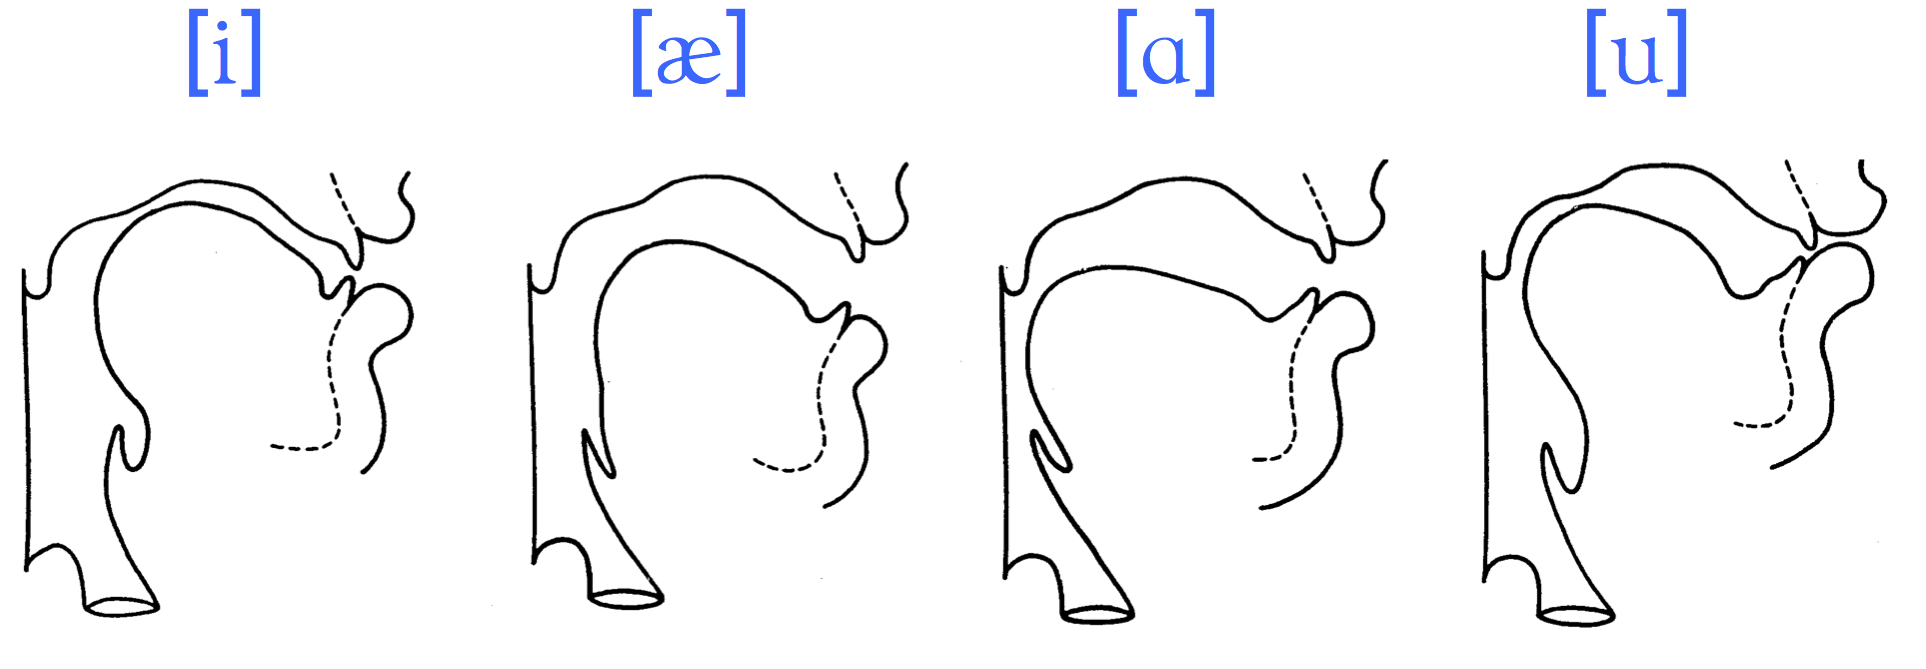
\includegraphics[scale=0.5]{Figures/vowels_prod.png}
    \caption{Vowels production \cite{mit_phonetics}}
    \label{fig:vowels_prod}
\end{figure}

\subsection{Vowel of American English}
\label{sub:vowel_of_american_english}
There are 18 different vowels in American English that can be grouped by three different sets: the \textbf{monopthongs}, the \textbf{diphthongs}, and the \textbf{schwa's} - or reduced vowels.

\begin{figure}[!ht]
    \centering
    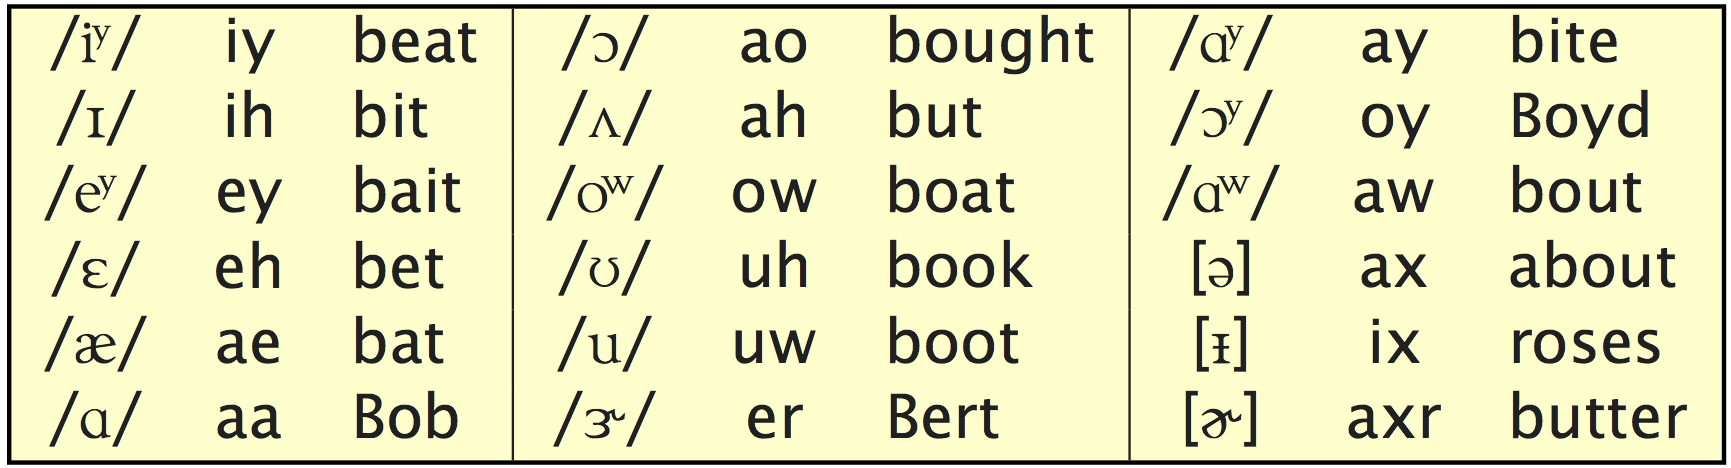
\includegraphics[scale=0.5]{Figures/vowels_sets.png}
    \caption{Example of words depending on the group \cite{mit_phonetics}}
    \label{fig:vowels_sets}
\end{figure}

The first column shows some examples of monopthongs. A \textit{monopthong} is a clear vowel sound in which the utterance are fixed at both the beginning and at the end. The central part of the picture represents the diphthongs. A \textit{diphthong} is the sound produced by two vowels when they occur within the same syllable. In the last column are depicted some examples of reduced vowels. \textit{Schwa's} refers to the vowel sound that stays in the mid-central of the word. In general, in English, the schwa is found in unstressed position.

%%%%%%%%%%%%%%%%%%%%%%%%%%%%%%%%%%%%%%%%%%%%%%%%%%%%%%%%%%%%%%%%%%%%%%%%%%%%%%%%%%%%%%%%%%%%%%%%%%%%%%%%%%%%%%%%%%%%%%%%%%%%%%%%%%

\subsection{Formants}
\label{sub:formants}
A \textit{formant} is the resonant frequency of a vocal track that resonate the loudest. In a spectrum graph, formants are represented by the peaks. In \ref{fig:peaks_formants} it is possible to see how the three first formants are defined by the peaks. The pictures is the \textit{envelope} of a spectrogram of the vowel \textbf{[i]}. Frequencies are the most relevant information to determine which vowel has been pronounced. In general, within a spectrum graph there may be a different number of formants, although the most relevant are the first three and they are named \textbf{F1}, \textbf{F2} and \textbf{F3}.

\begin{figure}[!ht]
    \centering
    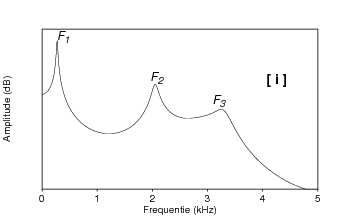
\includegraphics[scale=0.6]{Figures/peaks_formants.png}
    \caption{Spectral envelope of the [i] vowel pronunciation. F1, F2 and F3 are the first 3 formants \cite{formants_peaks}}
    \label{fig:peaks_formants}
\end{figure}

\noindent The frequencies produced by the formants are highly dependent on the tongue position. In fact, formant \textit{F1}'s frequencies are produced when the tongue is either in a \textit{high} or \textit{low} position, whereas formant \textit{F2} when the tongue is in either \textit{front} or \textit{back} position and formant \textit{F3} when the tongue is doing \textit{Retroflexion}. \textbf{Retroflection} is more present when pronouncing the consonant \textit{R}

%%%%%%%%%%%%%%%%%%%%%%%%%%%%%%%%%%%%%%%%%%%%%%%%%%%%%%%%%%%%%%%%%%%%%%%%%%%%%%%%%%%%%%%%%%%%%%%%%%%%%%%%%%%%%%%%%%%%%%%%%%%%%%%%%%

\subsection{Vowel duration}
\label{sub:vowel_duration}
The duration of a vowel is the time that taken when pronouncing it. The duration is measured in \textit{centiseconds} and in English\footnote{In Icelandic as well} the different lengths are defined by certain rules. In general, the length of \textit{lax vowels} such as /\textipa{I e \ae 2 6 u 9}/ are short whereas \textit{tense vowels} like /\textipa{i: A: O: u: 3:}/ including diphthongs /\textipa{eI aI OI 9U aU I9 ea U9}/ have a variable length but longer than lax vowels \cite{vowel_length}. In \ref{fig:vowel_length} is shown an example of time-length of some vowels.
\noindent In General American English, the length of vowels are not as distinctive as in the \textit{RP}\footnote{More commonly referred as the Standard English in the UK} pronunciation. In some American accents, to express an emphasis the length of vowels can be extended.

\begin{figure}[!ht]
    \centering
    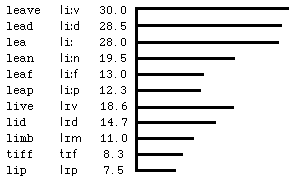
\includegraphics[scale=0.6]{Figures/vowel_length.png}
    \caption{RP vowel length \cite{vowel_length}}
    \label{fig:vowel_length}
\end{figure}

%%%%%%%%%%%%%%%%%%%%%%%%%%%%%%%%%%%%%%%%%%%%%%%%%%%%%%%%%%%%%%%%%%%%%%%%%%%%%%%%%%%%%%%%%%%%%%%%%%%%%%%%%%%%%%%%%%%%%%%%%%%%%%%%%%

\section{Fricative Production}
\label{sec:fricative_production}
A \textbf{fricative} is a consonant sound that is produced by narrowing the cavity causing a friction as the air goes through it \cite{fricatives}. There are eight fricatives in American English divided in two categories: \textit{Unvoiced} and \textit{Voiced}. These two categories are often called \textit{Non-Strident} and \textit{Strident} that means that there is a constriction behind the alveolar ridge.

\begin{figure}[!ht]
    \centering
    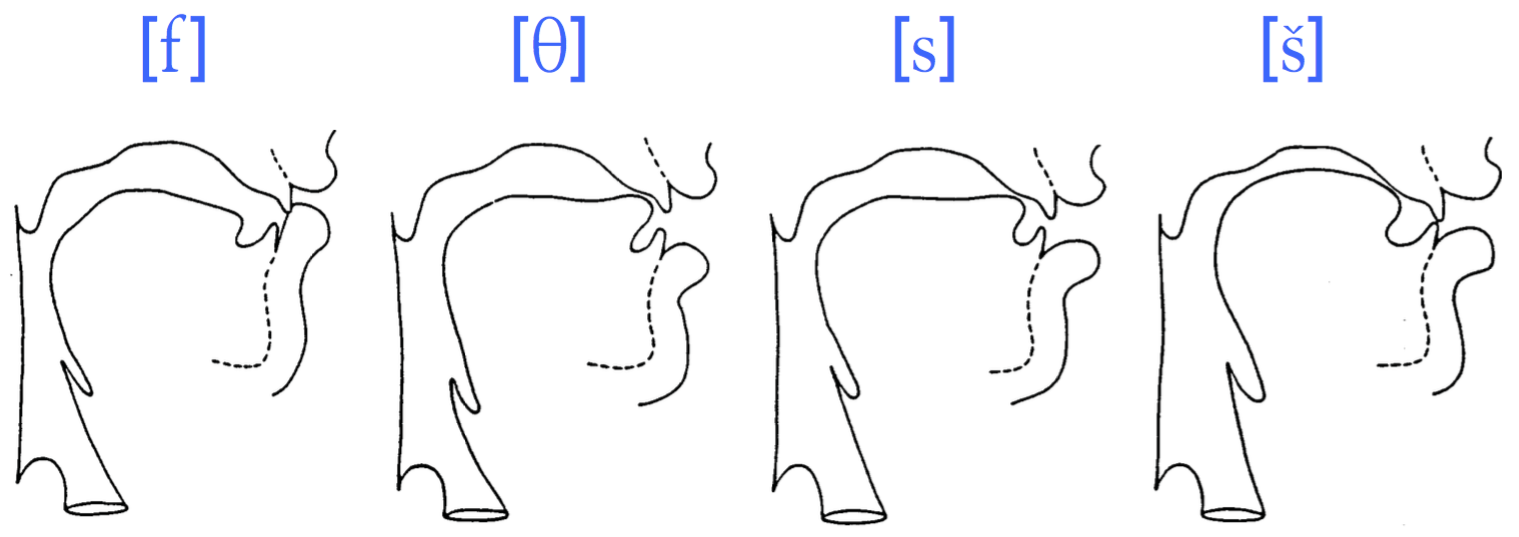
\includegraphics[scale=0.5]{Figures/fricative_production.png}
    \caption{Fricative production \cite{mit_phonetics}}
    \label{fig:fricative_prod}
\end{figure}

\noindent In \ref{fig:fricative_ex} it is possible to see some examples of these two categories. Each consonant also belongs to a specific articulation position. In fact, each figure in \ref{fig:fricative_prod} represents a specific articulation position. From left to right we have: \textit{Labio-Dental} (Labial), \textit{Interdental} (Dental), \textit{Alveolar} and \textit{Palato-Alveolar} (Palatal).

\begin{figure}[!ht]
    \centering
    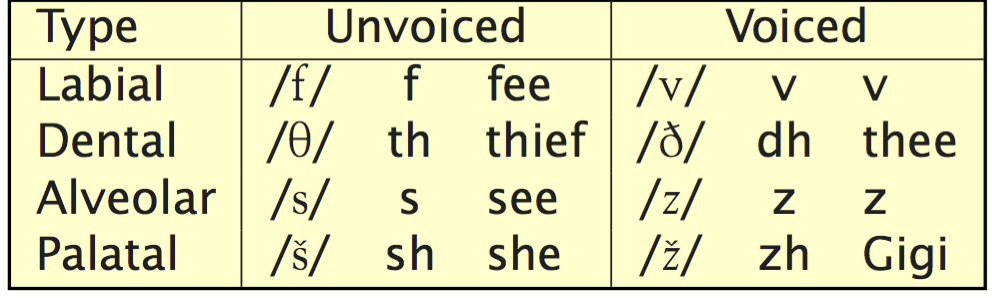
\includegraphics[scale=0.5]{Figures/fricative_examples.png}
    \caption{Fricative examples of productions \cite{mit_phonetics}}
    \label{fig:fricative_ex}
\end{figure}

%%%%%%%%%%%%%%%%%%%%%%%%%%%%%%%%%%%%%%%%%%%%%%%%%%%%%%%%%%%%%%%%%%%%%%%%%%%%%%%%%%%%%%%%%%%%%%%%%%%%%%%%%%%%%%%%%%%%%%%%%%%%%%%%%%

\section{Affricate Production}
\label{sec:Affricate Production}
An \textbf{affricate} consonant is produced by stopping the airflow first and then release it similar to a fricative. The result is also considered a \textit{turbulence noise} since the produced sound has a sudden release of the constriction. In English there only two affricate phonemes, as depicted in \ref{fig:affricate_prod}.

\begin{figure}[!ht]
    \centering
    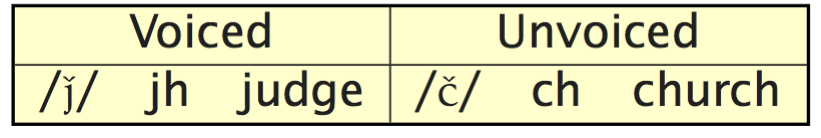
\includegraphics[scale=0.5]{Figures/affricative_production.png}
    \caption{Affricative production \cite{mit_phonetics}}
    \label{fig:affricate_prod}
\end{figure}

%%%%%%%%%%%%%%%%%%%%%%%%%%%%%%%%%%%%%%%%%%%%%%%%%%%%%%%%%%%%%%%%%%%%%%%%%%%%%%%%%%%%%%%%%%%%%%%%%%%%%%%%%%%%%%%%%%%%%%%%%%%%%%%%%%

\section{Aspirant Production}
\label{sec:Aspirant Production}
An \textbf{aspirant} consonant is a strong outbreak of breath produced by generating a turbulent airflow at glottis level. In American English exists only one aspirant consonant and it is the /\textipa{h}/, for instance in the word \textit{hat}.

%%%%%%%%%%%%%%%%%%%%%%%%%%%%%%%%%%%%%%%%%%%%%%%%%%%%%%%%%%%%%%%%%%%%%%%%%%%%%%%%%%%%%%%%%%%%%%%%%%%%%%%%%%%%%%%%%%%%%%%%%%%%%%%%%%

\section{Stop Production}
\label{sec:Stop Producton}
A \textbf{Stop} is a consonant sound formed by stopping the airflow in the oral cavity. The stop consonant is also known as \textit{plosive} which means that when the air is released it creates a small \textit{explosive} sound \cite{stop_consonants}. The occlusion can come up in three different variance as shown in \ref{fig:stop_prod}: from left to right we have a \textit{Labial} occlusion, the \textit{Alveolar} occlusion and the \textit{Velar} occlusion. The pressure built up in the vocal tract, determine the produced sound depending on which occlusion is performed.

\begin{figure}[!ht]
    \centering
    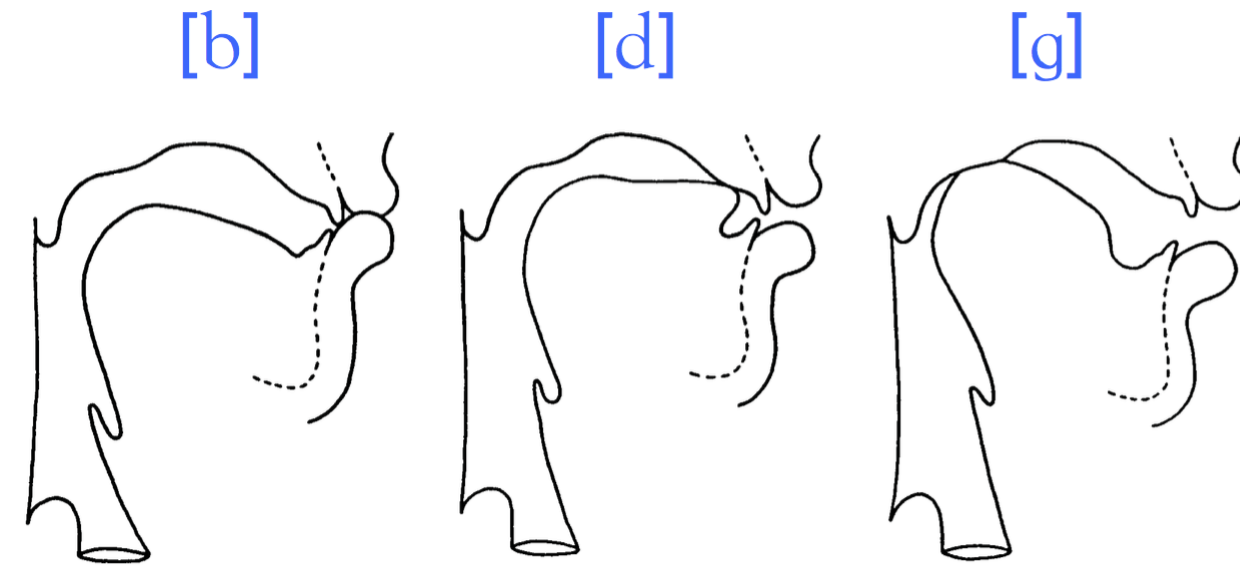
\includegraphics[scale=0.5]{Figures/stop_production.png}
    \caption{Stop production \cite{mit_phonetics}}
    \label{fig:stop_prod}
\end{figure}

\noindent In American English there are six stop consonants, as represented in \ref{fig:stop_ex}. As for the fricative consonants, the two main categories are the \textit{Voiced} and \textit{Unvoiced} sounds. Although, a particularity of the Unvoiced stops is that they are typically \textit{aspirated} whereas in the Voiced ones there is a \textit{voice-bar} during the closure movement. These two particularities are very useful where analyzing the formants because the frequencies are very well distinguished allowing a classification system to better understand the difference between stop phonemes.

\begin{figure}[!ht]
    \centering
    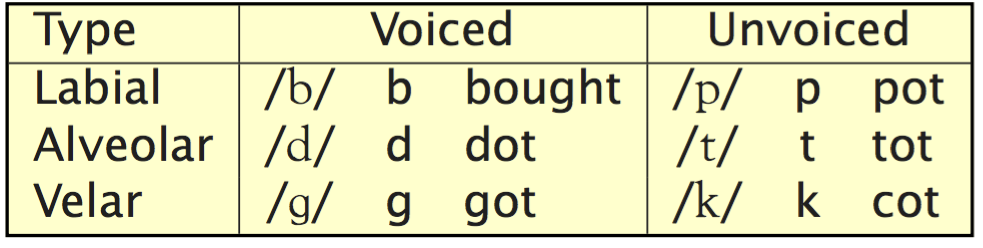
\includegraphics[scale=0.5]{Figures/stop_examples.png}
    \caption{Stop examples of production \cite{mit_phonetics}}
    \label{fig:stop_ex}
\end{figure}

%%%%%%%%%%%%%%%%%%%%%%%%%%%%%%%%%%%%%%%%%%%%%%%%%%%%%%%%%%%%%%%%%%%%%%%%%%%%%%%%%%%%%%%%%%%%%%%%%%%%%%%%%%%%%%%%%%%%%%%%%%%%%%%%%%

\section{Nasal Production}
\label{sec:Nasal Production}
A \textbf{Nasal} is an occlusive consonant sound that is produced with lowering of the soft palate \textit{(lowered velum)} at the back of the mouth, allowing the airflow to go out through the nostrils \cite{nasal_speech_sound}. Because the airflow escapes through the nose, the consonants are produced with a closure in the vocal tract. \ref{fig:nasal_prod} shows the three different positions to produce a nasal consonant. From left to right we have \textit{Labial}, \textit{Alveolar} and \textit{Velar}. \\
\noindent Due to this particularity, the frequencies of nasal \textit{murmurs} are quite similar. If we take a look on the spectrogram in \ref{fig:nasal_spectrogram}, it is possible to notice that nasal consonants have a high similarity. In a classification system, this can be a problem.

\begin{figure}[!ht]
    \centering
    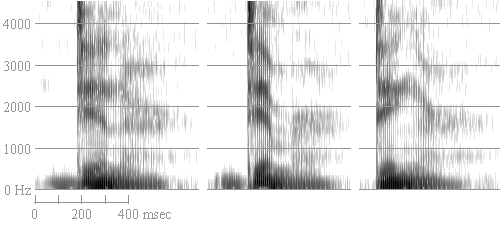
\includegraphics[scale=0.6]{Figures/nasal_spectrogram.png}
    \caption{Nasal Spectrograms of \textbf{dinner}, \textbf{dimmer}, \textbf{dinger} \cite{nasal_spectrogram}}
    \label{fig:nasal_spectrogram}
\end{figure}

\begin{figure}[!ht]
    \centering
    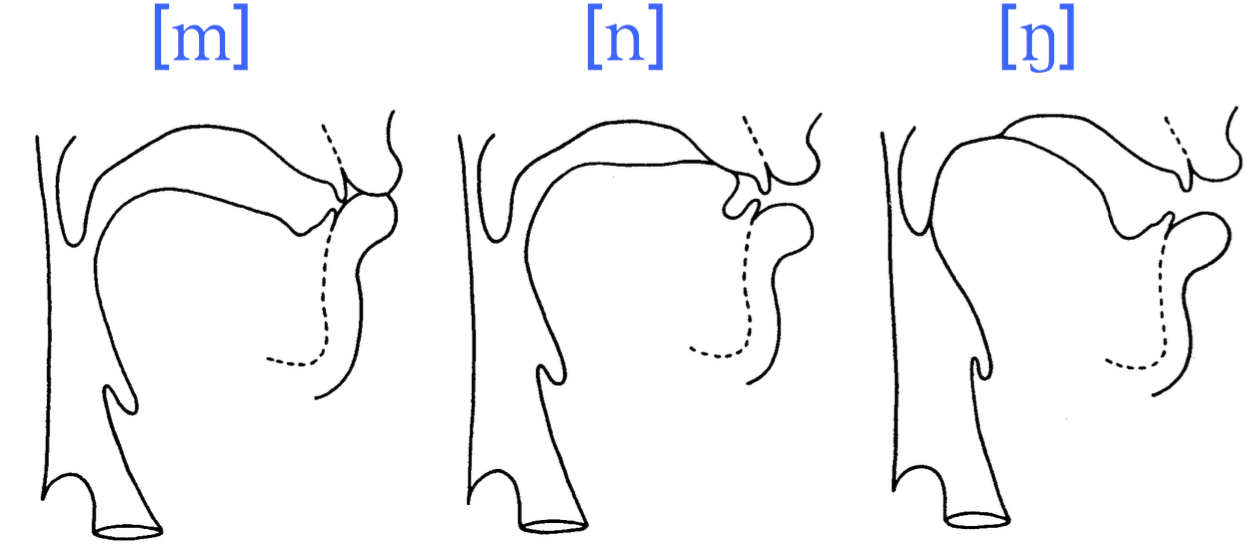
\includegraphics[scale=0.5]{Figures/nasal_production.png}
    \caption{Nasal production \cite{mit_phonetics}}
    \label{fig:nasal_prod}
\end{figure}

\noindent Since the sound produced by a nasal is produced with an occlusive vocal tract, each consonant is \textbf{always attached} to a vowel and it can form an entire syllable. Although, in English, the consonant /\textbf{\textipa{N}}/ always occur immediately after a vowel. In \ref{fig:nsal_ex} are shown some examples of nasal consonants divided by articulation position.

\begin{figure}[!ht]
    \centering
    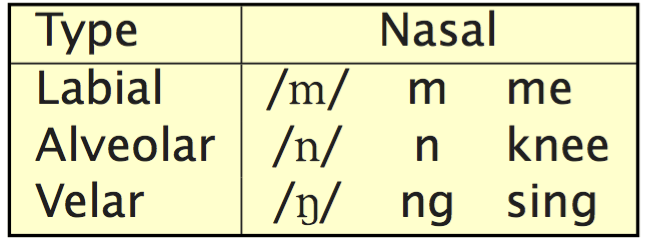
\includegraphics[scale=0.5]{Figures/nasal_examples.png}
    \caption{Nasal examples of production \cite{mit_phonetics}}
    \label{fig:nsal_ex}
\end{figure}

%%%%%%%%%%%%%%%%%%%%%%%%%%%%%%%%%%%%%%%%%%%%%%%%%%%%%%%%%%%%%%%%%%%%%%%%%%%%%%%%%%%%%%%%%%%%%%%%%%%%%%%%%%%%%%%%%%%%%%%%%%%%%%%%%%

\section{Semivowels Production}
\label{sec:Semivowels Production}
A \textbf{semivowel} is a sound that is very close to a vowel sound but it works more likely as a syllable boundary rather than a core of a syllable \cite{ladefoged1998sounds}. A typical example of semivowels in English are the \textbf{y} and \textbf{w} in words \textit{yes} and \textit{west}. In the \textit{IPA} alphabet they are written /\textipa{j}/ and /\textipa{w}/ and they correspond to the vowels /\textipa{i:}/ and /\textipa{u:}/ in the words \textit{seen} and \textit{moon}. In \ref{fig:semivowel_ex} there are some examples of semivowels production. \\
\noindent The sound is produced by making a constriction in the oral cavity without having any sort of air turbulence. To achieve that, the articulation motion is slower than other consonants because the laterals\footnote{They are a pair of upper teeth that are located laterally from the central incisors \cite{laterals_wiki}} form a complete closer combined with a tongue tip. In this way the airflow has to pour out using the sides of the constriction.

\begin{figure}[!ht]
    \centering
    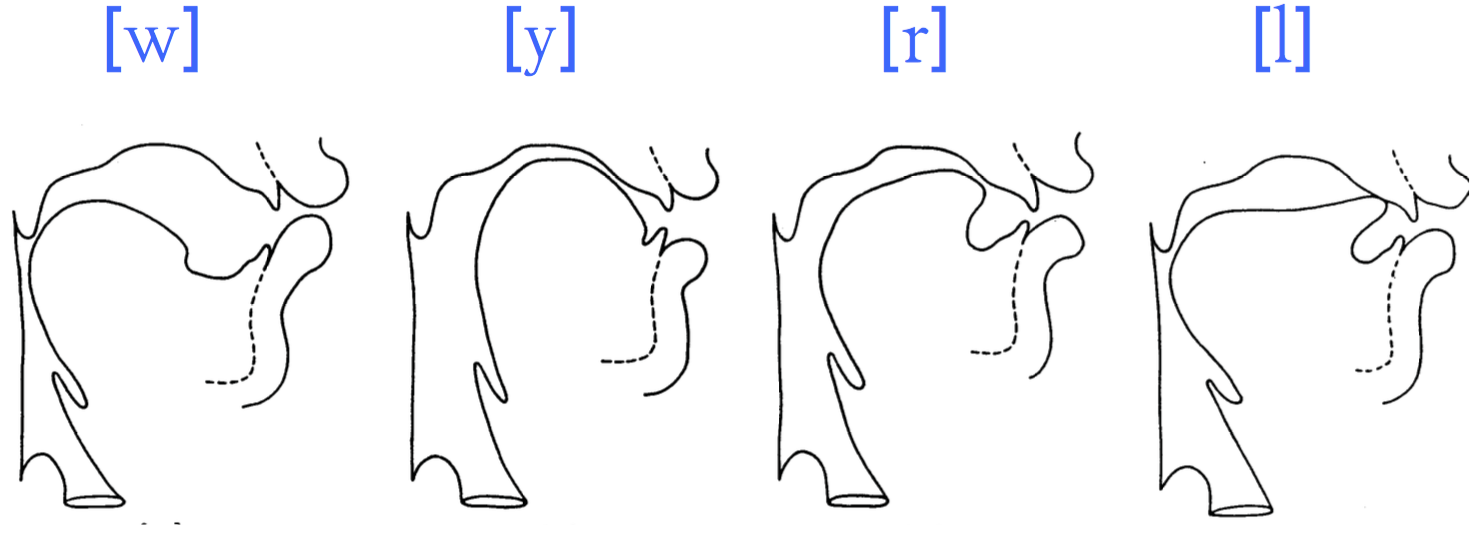
\includegraphics[scale=0.5]{Figures/semivowel_production.png}
    \caption{Semivowel production \cite{mit_phonetics}}
    \label{fig:semivowel_prod}
\end{figure}

\noindent In American English there are four semivowels and they are depicted in \ref{fig:semivowel_prod}. An important fact of semivowels is that they are always close to a vowel. Although, the /\textipa{l}/ can form an entire syllable by itself when there is no stress in a word.

\begin{figure}[!ht]
    \centering
    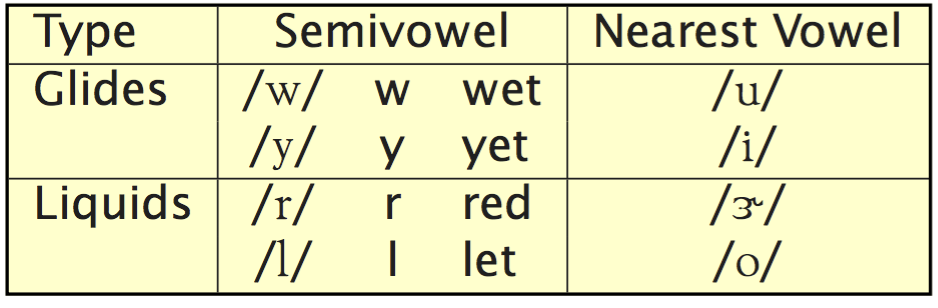
\includegraphics[scale=0.5]{Figures/semivowel_examples.png}
    \caption{Semivowel examples of production \cite{mit_phonetics}}
    \label{fig:semivowel_ex}
\end{figure}

%%%%%%%%%%%%%%%%%%%%%%%%%%%%%%%%%%%%%%%%%%%%%%%%%%%%%%%%%%%%%%%%%%%%%%%%%%%%%%%%%%%%%%%%%%%%%%%%%%%%%%%%%%%%%%%%%%%%%%%%%%%%%%%%%%

\subsubsection{Acoustic Properties of Semivowels}
\label{ssub:Acousitc Properties of Semivowels}
Semivowels have some properties that are taken into account when doing any sort of analysis. In fact, /\textipa{w}/ and /\textipa{l}/ are the semivowels that are more confusable because both are characterized by a \textit{low} range of frequencies for both formants \textit{F1} and \textit{F2}. Although, the /\textipa{w}/ can be distinguished by the \textit{rapid falloff} in the F2 spectrogram whereas /\textipa{l}/ has more often a \textit{high frequency energy} compared to /\textipa{w}/. The \textbf{energy} is the relationship between the \textit{wavelength} and the \textit{frequency}. So, having a high energy means that there is a high frequency value and a small wavelength \cite{energy_relationship}. \\
\noindent The semivowel /\textipa{y}/ is characterized by having a very low frequency value in formant F1 and a very high in formant F2. The /\textipa{r}/ instead is presented with a very low frequency value of formant F3. \\


%%%%%%%%%%%%%%%%%%%%%%%%%%%%%%%%%%%%%%%%%%%%%%%%%%%%%%%%%%%%%%%%%%%%%%%%%%%%%%%%%%%%%%%%%%%%%%%%%%%%%%%%%%%%%%%%%%%%%%%%%%%%%%%%%%

\section{The Syllable}
\label{sec:The syllable}
The definition of the \textbf{syllable} can be divided in two sub-definition: one from the phonetic point of view and one from the phonological point of view. \\
\noindent In phonetic analysis, the syllable is a basic unit of speech in which they \textit{"are usually described as consisting of a centre which has little or no obstruction to airflow and which sounds comparatively loud; before and after that centre (...) there will be greater obstruction to airflow and/or less loud sound"} \cite{roach2000phonology}. Taking the word \textit{cat} (/\textipa{k\ae t}/) as example, the \textbf{centre} is defined by the vowel /\textipa{\ae}/ in which takes place only a little obstruction. The surrounding \textit{plosive} consonants (/\textipa{k}/ and /\textipa{t}/) the airflow is completely blocked \cite{syllable_site}. \\
\noindent A phonological definition of the syllable establishes that it is \textit{"a complex unit made up of nuclear and marginal elements"}\cite{laver1994principles}. In this context, the vowels are considered the \textbf{Nuclear} elements or syllabic segments whereas the \textbf{Marginal} ones are the consonants or non-syllabic segments \cite{syllable_site}. Considering the word \textit{paint} (/\textipa{peInt}/) as example, the nuclear element is defined by the diphthong /\textipa{eI}/ whereas /\textipa{p}/ and /\textipa{nt}/ are the marginal elements.

\subsection{Syllable Structure}
In the phonological theory, the syllable can be decomposed in a hierarchical structure instead of a linear one. The structure starts with the $\sigma$ letter in which represents not only the root, but the syllable itself. Immediately after, there are two \textit{branches} called \textbf{constituents} that they represents the \textit{Onset} and the \textit{Rhyme}. The left branch includes any consonants that precede the vowel (or Nuclear element), whereas the right branch includes both the nuclear element and any consonants (or Marginal elements) that potentially could follow it. \\
\noindent Usually, the rhyme branch is further split in two other branches represented by the \textbf{Nucleus} and the \textbf{Coda}. The first on represent the nuclear element in the syllable. The second one instead, subsumes all the consonants that follow the Nucleus in the syllable \cite{syllable_site}. In \ref{fig:syllable_structure} there is a representation of the syllable structure based on the word \textit{plant}.

\begin{figure}
    \begin{center}
        \fbox{
            \begin{forest}
              for tree={
                parent anchor=south,
                child anchor=north,
                align=center,
                if n children=0{
                  font=\itshape,
                  tier=terminal,
                }{},
              }
              [$\sigma$
                [onset [CC [\textipa{pl}]]]
                [rhyme [Nucleus [V [\textipa{\ae}]]][Coda [C [\textipa{nt}]]]]
              ]
            \end{forest}
        }
    \end{center}
    \caption{Tree structure of the word \textbf{plant}\protect\footnotemark}
    \label{fig:syllable_structure}
\end{figure}

\footnotetext{\textbf{C} means \textit{Consonant} whereas \textbf{V} means \textit{Vowel}}

\chapter{Acoustics and Digital Signal Processing}
\label{ch:speech analysis}
In the past decade, digital computers have significantly helped \textit{signal processing} to quantify a finite number of bits. The flexibility inherited from digital elements allowed the usage of a vast number of techniques in which had been not possible to implement in the past. Nowadays, digital signal processor have been used to perform multiple operations, such as \textit{filtering}, \textit{spectrum estimation} and many others algorithms \cite{orfanidis1995introduction}.


\section{Speech signals}
\label{sec:speech_signals}
The \textbf{speech} is the human way of communication. The protocol used in communication is based on a syntactic combination of different words taken from a very large vocabulary. Each word in the vocabulary is composed by a small set of vowels and consonants that combined with a phonetic units form a spoken word. \\
\noindent When a word is pronounced\footnote{\ref{ch:english_language} explains in details how phonemes are pronunced}, a sounds is produced causing the air particles to be excited at a certain vibration rate. The source of our voice is due to the vibration of the vocal cords. The resultant signal is a \textit{non-stationary} but it can be divided in segments since each phoneme has a common acoustic properties. In \ref{fig:ex_sound_wave} is possible to notice how the pronounced words have a different shape as well as when the intensity of the voice is higher/lower during the pronunciation.
 
\begin{figure}[!ht]
	\centering
	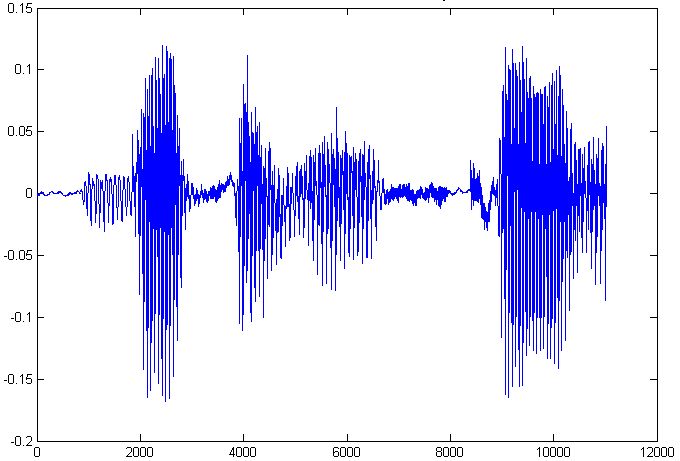
\includegraphics[scale=0.4]{Figures/ex_speech.png}
	\caption{Example of a speech sound. In this case, the sentence "This is a story" has been pronounced \cite{ex_speech_image}}
	\label{fig:ex_sound_wave}
\end{figure}

\noindent The simplest form of sound is the \textit{sinusoid} and it is the easiest waveform to describe because it corresponds to a \textbf{pure tone}. A pure tone consist in a waveform that consists only on one frequency. Other examples are the \textit{cosine} or \textit{sine} waves.

\subsection{Properties of Sinusoids}
\label{sub:prop_of_sinusoids}
A sinusoid, is a simple waveform represented by a up and down movement. There are three important measures that has to be taken into consideration when defining the shape of the sinusoid: \textit{amplitude}, \textit{frequency} and \textit{phase}. 

\subsubsection{Amplitude}
The amplitude, from a sound point of view, corresponds to the \textit{loudness} whereas in the soundwave it corresponds to the amount of \textbf{energy}. In general, to measure the amplitude, we use the unit called \textbf{deciBels} (dB) in which it is measured using a logarithmic scale relative to a standard sound \cite{prop_of_sinusoids}.

\subsubsection{Frequency}
Frequency is the number of cycles per unit of time\footnote{In general, a unit of time is considered a single second}.To define cycle, we can think of an oscillation that starts from the middle line, goes to the maximum point, down to the minimum and get back to the middle point. The unit of measure of the frequency is calculated in \textbf{Hertz} (Hz). Also, if we calculate the time taken for one cycle, we estimate the so called \textbf{period}. \\ 
\noindent Frequency plays a fundamental role with the \textit{pitch}. In fact, changing the number of oscillations but keeping the same waveform, we are able to increase or decrease the level of the pitch.

\subsubsection{Phase}
The \textbf{phase} measures the starting point position of the waveform. If the sinusoids start at the very minimum of the wave, the value of the phase is $\pi$ radians whereas starting from the top of the wave it will have a phase of \textit{zero}. When two sounds do not have the same phase, it is possible to perceive the difference in the time scale since one of the two is delayed compared to the other. When comparing two signals, there is the need to obtain a \textit{"phase-neutral"} that means the comparison is made taking only into account Amplitude and Frequency. This method is called \textbf{autocorrelation} of the signals.

\subsection{Spectrograms}
\label{sec:spectrograms}
A \textbf{Spectrogram} is the visual representation of an acoustic signal \cite{spectrogram_def}. Basically, a Fourier Transformation is applied to the sound, in such a way to obtain the set of waveforms extracted form the original signal and separate their frequencies and amplitudes. The result is typically depicted in a graph with degrees of amplitude with a \textit{light-dark} representation. Since amplitude represents the \textit{energy}, having a darker shade means that the energy is more intense in a certain range of frequencies - lighter when there is low energy. In \ref{fig:nasal_spectrogram} there is an example of the spectrogram. \\
\noindent The visual feedback of the spectrogram is highly dependent from the \textbf{window size} of the Fourier Analysis. In fact, different sizes affect the levels of frequencies and time resolution. \\
\noindent If the window size is \textit{short}, the adjacent \textbf{harmonics} are distorted but the time resolution is better \cite{spectrogram_def}. An harmonic is \textit{"an integer multiple of the fundamental frequency"}\cite{harmonic_wiki} or component frequencies. This is helpful when we are looking for the \textit{formant structure} because the striations created by the spectrogram highlights the individual pitch periods. \\
\noindent On the other hand, a \textit{wider} window size, helps to locate the harmonics because the band of the spectrogram are narrower.


\section{Fourier Analysis}
\label{sec:fourier_analysis}
\textbf{Fourier Analysis} is the process that decompose a periodic waveform into a set of sinusoids having different amplitudes, phases and frequencies. Yet, if we add those waveforms again, we will obtain the original signal. The analysis has been involved in many scientific applications and the reason is due to the following transform properties:

\begin{itemize}
	\item Linear transformation - the relationship between two modules is kept
	\item Exponential function are eigenfunctions of differentiation \cite{evans1997partial}
	\item Invertible - derived from the linear relationship
\end{itemize}

\noindent In signal processing, the Fourier analysis is used to isolate singular components of a complex waveform. A set of techniques consist in using \textbf{Fourier Transformation} on a signal in such a way to be able to manipulate the data in the easiest way possible but at the same time we have to be capable of inverting the transformation \cite{fa_wiki} \cite{rabiner1975theory}. In the next subsections we describe the fundamental steps for manipulating a signal.

\subsubsection{Sampling}
\label{ssubs:sampling}
\textit{Sampling} is the process that transform a continuous signal in to a discrete one. Each sample can be either be a single value or a set of values at a certain point in time \cite{sampling_wiki}. \\ 
\noindent Consider a sound signal that varies in time a continuous function $s(t)$. For every $T$ seconds, we need to measure the value of the function. This frame of time is called the \textit{sampling intervar} \cite{weik2012communications}. To calculate the sequence a sampled function is given as follow: $s(nT), \forall$ integer values of $n$. Thus, the \textit{sampling rate} is the average number of samples obtained in a range of $T = 1sec$ \cite{sampling_wiki}. An example of sampling is shown in \ref{fig:sampling_ex}.

\begin{figure}[!ht]
	\centering
	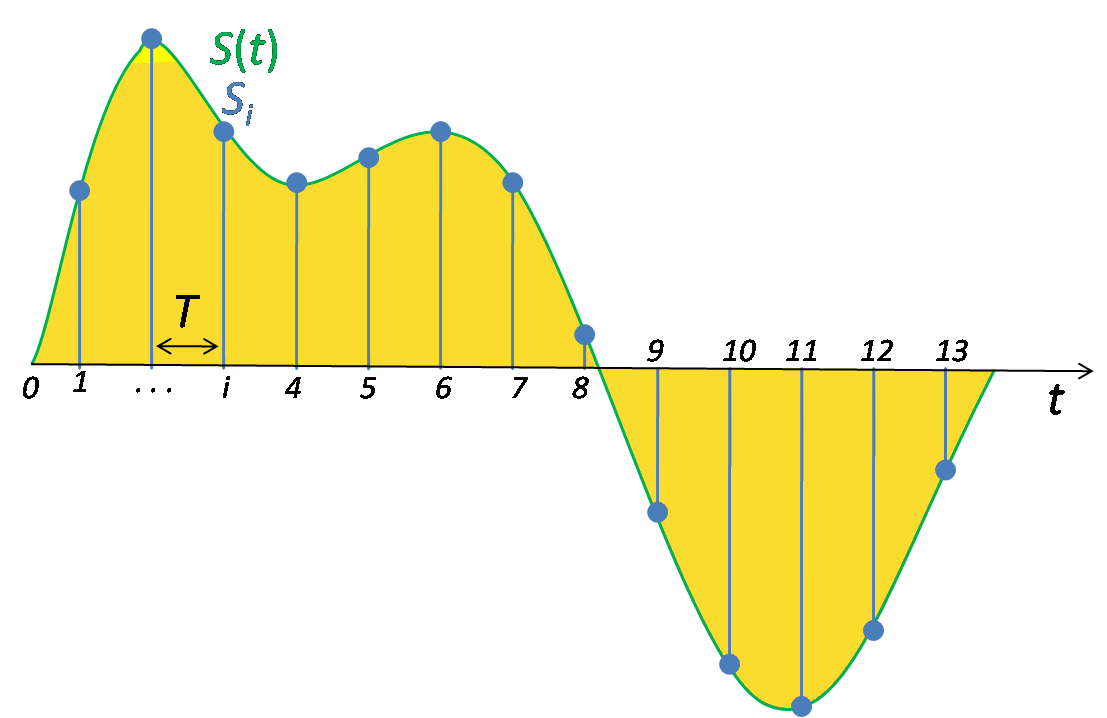
\includegraphics[scale=0.2]{Figures/sampling_example.png}
	\caption{Example of signal sampling. The green line represents the constinuous signal whereas the samples are represented by the blu lines \cite{sampling_wiki}}
	\label{fig:sampling_ex}
\end{figure}

\noindent As we mentioned above, using the Fourier Analysis we need to be able to reconstruct the original signal from the transformed one. To be able to, the \textbf{Nyquist-Shannon} theorem states that the sampling rate has to be larger as twice as the maximum frequency of the signal, in order to rebuild the original signal \cite{sampling_illinois}.\\
\noindent The \textit{Nyquist sampling rate} is defined by the following equation:

\begin{equation}
f_{s} > f_{Nyquist} = 2f_{max}
\end{equation}


\subsubsection{Quantization}
\label{subs:quantization}
To finalize the transformation from a continuous signal to a discrete one, we need to \textit{quantized} the signal in such a way to obtain a finite set of values. Unlike sampling in which permits to reconstruct the original signal, quantization is an irreversible operation that introduce a loss of information. \\
\noindent Consider $x$ be the sampled signal and $x_{q}$ the quantized one where $x_{q}$ can be expressed as the signal $x$ plus the error $e_{q}$. From here we have:

\begin{equation}
x_{q} = x + e{q} \Leftrightarrow e_{q} = x - x_{q}
\end{equation}

Given the equation above, we can restrict the range of error to $-q/2 ... +q/2$ because we will not make a larger error than the half of the quantization step. From a mathematical point of view, the error-signal is a random signal with an uniform probability distribution between the range of $−q/2 and +q/2$, giving the following \cite{quantization_math}:

\begin{equation}
p(e) = \begin{Bmatrix}
			\frac{1}{q} & for \frac{-q}{2} \leq  e < \frac{q}{2}\\ 
			0 			& otherwise
		\end{Bmatrix}
\end{equation}

Given this reason, the quantization error also called quantization noise.

\subsubsection{Windowing Signals}
\label{ssubs:windowing_signals}


\subsubsection{Zero Crossing Rate}
\label{ssubs:Zero Crossing Rate}


\subsubsection{Autocorrelation}
\label{ssubs:autocorrelation}



\section{Frequency Domain Analysis}
\label{sec:freq_domain_analysis}


\subsection{The Discrete Fourier Transform}
\label{sub:discrete_fourier_transform}

\chapter{Speech Recognition}
\label{chap:Speech Recognition}
Speech recognition is a sub-field of machine learning in which allows a computer program to extract and recognize words or sentences from a human being language, and converting them back to a machine language. Advance techniques nowadays, permits to understand natural speech for executing tasks. Google Voice Search\footnote{\url{https://www.google.com/search/about/}} and Siri\footnote{\url{http://www.apple.com/ios/siri/}} are two examples of very advance speech recognition softwares with the capability of understanding natural language.

\section{The Problem of Speech Recognition}
\label{sec:The Problem of Speech Recognition}
Human languages are very complex and different among each other. Despite they might have a well-structured grammar, automatically recognition is still a very difficult problem since people have many ways to say the same thing. In fact, spoken language is different from written one because the articulation of verbal utterance is less strict and complicated. \\
The environment in which the sound is taken has a big influence on the speech recognition software because it introduces a \textit{unwanted} amount of information in the signal. For this reason it is important that the system is capable of \textit{identifying} and \textit{filtering out} this surplus of information \cite{forsberg2003speech}. \\

\noindent Another interesting set of problems are related to the speaker itself. Each person has a different body that means there are a variety of components that the recognition system has to take care of in such a way to be able to understand correctly. Gender, vocal tracts, speaking style, speed of the speech, regional provenience are fundamental parts that have to be taken in consideration when building the \textit{acoustic model} for the system. Despite these features are unique for each person, there some common aspects that will be used to construct the model. The acoustic model represents the relationship between the acoustic signal of the speech and the phonemes related to it. \\

\noindent Ambiguity represents the major concern since natural languages have inherited it. In fact, it may happen that in a sentence we are not able to discriminate which words are actually intended \cite{forsberg2003speech}. In speech recognition there are two types of ambiguity: \textit{homophones} and \textit{word boundary ambiguity}. \\
Homophones refers to those words that are spelled in a different way but they \textbf{sound} the same. Generally speaking, these words are not correlated to each other but it happened that the sound is equivalent. Word boundary ambiguity instead, it \textit{occurs when there are multiple ways of grouping phones into words}\cite{forsberg2003speech}.

% CMU Sphinx4
\section{Architecture}
\label{sec:speech_rec_Architecture}
Generally speaking, a speech recognition system is divided in three main components: the \textbf{Feature Extraction} (or Front End), the \textbf{Decoder} and the \textbf{Knowledge Base} (KB). In \ref{fig:speech_architecture} the KB part is represented by the three sub-blocks called \textit{Acoustic Model}, \textit{Pronunciation Dictionary} and \textit{Language Model}. The \textit{Front End} takes as in input the voice signal where it is analyzed and converted in the so called \textit{Features Vectors}. This last is the set of common properties that we discussed in \ref{ch:english_language}. From here we can say that $\textbf{Y} 1:N = y_{1},..., y_{N}$ where $Y$ is the set of features vectors. \\
The second step consists in feeding the \textit{Decoder} with vectors we obtained from the previous step, attempting to find the sequence of words $\textbf{w} 1:L = w_{1}, ... , w_{L}$ that have most likely generated the set $Y$\cite{gales2008application}. The decoder tries to find the likelihood estimation as follows:

\begin{equation}
	\widehat{w} = \underset{w}{arg max} P(\textbf{w}| \textbf{Y})
\end{equation} 

\noindent The $P (w|Y)$ is difficult to find directly\footnote{There is discriminate way of finding the estimation directly as described in \cite{gales2007discriminative}}, but using Bayes' Rules we can transform the equation above in

\begin{equation}
	\widehat{w} = \underset{w}{arg \; max} P (\textbf{Y}|\textbf{w}) P(\textbf{w})
\end{equation}

\noindent in which the probability $P(Y|w)$ and $P(w)$ are estimated by the \textit{Knowledge Base} block. In particular, the \textit{Acoustic Model} is responsible to estimate the first one whereas the \textit{Language Model} estimates the second one. \\
\noindent Each word \textbf{w} is decomposed in smaller components called \textit{phones}, representing the collection of phonemes $\textbf{K}_{w}$ (see \ref{ch:english_language}). We can describe the \textit{pronunciation} as $\overset{(w)}{\textbf{q}_{1:K_{w}}} = q_{1}, ...., q_{K_{w}}$. The likelihood estimation of the sequence of phonemes is calculated by a \textbf{Hidden Markov Model} (HMM). In the section, a general overview of HMM is given. We are not going to discuss a particular model because every speech recognition system uses a variation of the general HMM chain. \\

\begin{figure}[!ht]
	\centering
	\includegraphics[scale=0.8]{Figures/speech_Architecture.png}
	\caption{HMM-Based speech recognition system \cite{gales2008application}}
	\label{fig:speech_architecture}
\end{figure}

\section{Hidden Markov Model}
\label{sec:hmm}
\noindent A definition given by \cite{eddy1996hidden} is the following: \textit{"An Hidden Markov Model is a finite model that describes the probability distribution over an infinite number of possible sequences"}. Each sequence is determined by a set of \textit{transition probabilities} in which describes the transitions among states. The \textbf{observation} (or outcome) of each state is generated based on the associated probability distribution. From an \textit{outside} perspective, the \textit{observer} is only able to see the outcome and not the state itself. Hence, the states are considered \textbf{hidden} which leads to the name Hidden Markov Model \cite{def_hmm}. \\

\noindent An HMM is composed by the following elements:

\begin{itemize}
	\item The number of states (N)
	\item The number of observations (M), that becomes infinite if the set of observations is contiguous
	\item The set of transition probabilities, $\Lambda = \{ a_{ij}\}$
\end{itemize}

The set of probabilities is defined as follow:
\begin{equation}
\label{eq:transition_probabilities}
a_{ij} = p \, \{ \, q_{t+1} = j \, | \, q_{t} = i \, \}, \, \, \, 1 \leq i,j \leq N, 
\end{equation}

\noindent where $q_{t}$ is the state we are currently in and $a_{ij}$ represent the transition from state $i$ to $j$. 
Each transition should satisfy the following rules:

\begin{subequations}
	\label{eq:stochastic_rules}
	\begin{align}
	a_{ij} \geq 1, \, \, \, 1 \leq i,j \leq N, \\
	\sum_{j=1}^{N} a_{ij} = 1, \, \, \, 1 \leq j \leq N
	\end{align}
\end{subequations}

\noindent For each state $S$ we can define the probability distribution $S = \{s_{j}(k)\}$ as follow:

\begin{equation}
s_{j}(k) = p \, \{\, o_{t} = v_{k} \, | \, q_{t} = j \, \}, \, \, \, 1 \leq j \leq N, \,\, 1 \leq k \leq M
\end{equation}

\noindent where $v_k$ is the $k^{th}$ observation whereas $o_{t}$ is the outcome. Furthermore, $b_{j}(k)$ must satisfy the same stochastic rules described in \ref{eq:stochastic_rules}. \\

\noindent A different approach is made when the number of observations is infinite. In fact, we are not going to use a set of discrete probabilities but instead a continuous probability density function. Given that, we can define the parameters of the density function by approximating it by a weighted sum of $M$ Gaussian distributions $\varphi$ \cite{def_hmm}. We can describe the function as follow:

\begin{equation}
	s_{j}(o) = \sum_{m = 1}^{M} c_{jm}\varphi (\mu_{jm}, \Sigma_{jm}, o_{t})
\end{equation}

\noindent where $c_{jm}$ is the weighted coefficients, $\mu_{jm}$ is the mean vector and $\Sigma_{jm}$ is the covariance matrix. The coefficients should satisfy the stochastic rules in \ref{eq:stochastic_rules}. \\
\noindent We can then define the initial state distribution as $\pi = \{\pi_{i}\}$ where 

\begin{equation}
	\pi_{i} = p \, \{ q_{I} = i \, \}, \,\,\,\, 1 \leq i \leq N
\end{equation} 

\noindent Hence, to describe the HMM with the discrete probability function we can use the following compact form
\begin{equation}
\label{eq:hmm_discrete}
	\lambda = (\Lambda, S, \pi )
\end{equation}

\noindent whereas to denote the model with a continuous density function, we use the one described in \ref{eq:hmm_density}
\begin{equation}
\label{eq:hmm_density}
\lambda = (\Lambda, c_{jm}, \mu_{jm}, \Sigma_{jm}, \pi )
\end{equation} 

\subsection{Assumptions}
\label{sub:assumptions_hmm}
The theory behind HMM requires three important assumptions: the \textbf{Markov assumption}, the \textbf{stationarity assumption} and the \textbf{output independence assumption}.

\subsubsection{The Markov Assumption}
The Markov assumption assumes that the following state depends only from the state we are currently in as given in \ref{eq:transition_probabilities}. The result model is also referred as \textit{first order} HMM. Generally speaking though, the decision of the next coming state might depend on \textbf{n} previous states, leading to a $n^{th}$ HMM order model. In this case, the transition probabilities is defined as follow:

\begin{equation}
\label{eq:transition_nth_order}
a_{i_{1}i_{2}...i_{n}j} = p\, \{\, q_{t+1} = j \,|\, q_{t} = i_{1}, \, q_{t-1} = i_{2}, ... , \, q_{t-k+1} = i_{k} \, \}, \,\,\,\, 1 \leq i_{1},i_{2}, ... ,i_{k}, j \leq N
\end{equation}


\subsubsection{The Stationary Assumption}
The second assumption states that the transition probabilities are \textit{time-independent} when the transitions occur. This is defined by the following equation for any $t_{1}$ and $t_{2}$:

\begin{equation}
	p \, \{\, q_{t+1} = j \,|\, q_{t_{1}} = i\, \}\, = \,p \,\{\, q_{t_{2}+1} = j \,|\, q_{t_{2}} = i\, \}
\end{equation}

\subsubsection{The Output Assumption}
The last assumption says that the current observation is statistically independent from the previous observations. Let's consider the following observations:

\begin{equation}
	O = o_{1}, o_{2}, ... , o_{T}
\end{equation}

Now, recalling \ref{eq:hmm_discrete}, it is possible to formulate the assumption as follow:

\begin{equation}
	p \, \{\, O \, |\, q_{1},q_{2}, ... , q_{T}, \lambda \,\}\, = \, \prod_{t = 1}^{T} p \, \{ \, o_{t} \, | \, q_{t}, \, \lambda \,\}
\end{equation}

\section{Evaluation problem}


\subsection{Forward Algorithm}


\subsection{Backward Algorithm}


\section{Viterbi Algorithm}
\label{sec:viterbi}
Decoding part

\section{Maximum likelihood estimation}
\label{sec:mle}
Training the HMM



% GMM classifier
\section{\Naive Bayes and Gaussian models for classification}
\label{sec:Gaussian Classifiers and Distance Measures}

%\chapter{Artificial Neural Networks}
\section{Artificial Neuron}
Our brain is composed by biological neurons and an artificial neuron (or AN) is a representation of it. Every AN can gather signals from other nurons or from the environment, and after an elaboration it transmits another signal to all the other ANs that are connected to it \cite{engelbrecht2007computational}. A rapresentation of AN is depicted in \ref{fig:artificial_neuron}. \\
Each connection to the artificial neuron has a numerical weigth associated to it in which the input signal is hold back. The value of the weight can be either positive or negative. In most cases, the sums of each node are weighted and then given as input to a \textit{non-linear} function called \textbf{transfer function} or \textbf{activation function} \cite{artificial_neuron_wiki}. The activate function defines the output value of the node and typically, the \textit{Step Function}, \textit{Sigmoid Function} and a \textit{Softmax Function} are the most used.

\begin{figure}[!ht]
    \centering
    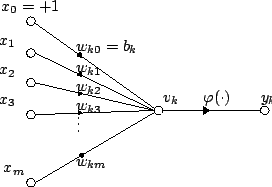
\includegraphics[scale=0.5]{Figures/artificial_neuron.png}
    \caption{Representation of an Artificial Neuron \cite{artificial_neuron_wiki}}
    \label{fig:artificial_neuron}
\end{figure}

\noindent From the mathematical point of view, we can define an artificial neuron as follow: \\
given $m+1$ inputs with signals from $x_1$ to $x_m$ and weights values from $w_0$ to $w_m$. The \textit{bias} is then defined by the input $x_0$ in which a value of 1 will be assigned. The bias value allows us to \textit{shift} the curve of the activation function to a certain direction and it is defined with $w_{k0} = b_k$ \cite{artificial_neuron_wiki}. \\
The output of the AN is:

\begin{equation*}
    y_k = \varphi \left ( \sum_{j=0}^{m} w_{kj} x_j \right )
\end{equation*}

\section{Network Function}
When there are many aritificial neurons interconnected between each other in the different layers, we form a \textit{network}. \ref{fig:ann} shows an example of ANN where the \textbf{inputs} are represented by the first layer in which they send data through the connection to the second group of neuron. The connection between two neuros is called \textit{synapses} where the \textbf{weigth} is stored. The second layer is connected to the third one that represents the \textbf{output} of the network. There can be multiple stratums between the inputs and the outputs and these are called \textit{hidden layers}. \\

\begin{figure}[!ht]
    \centering
    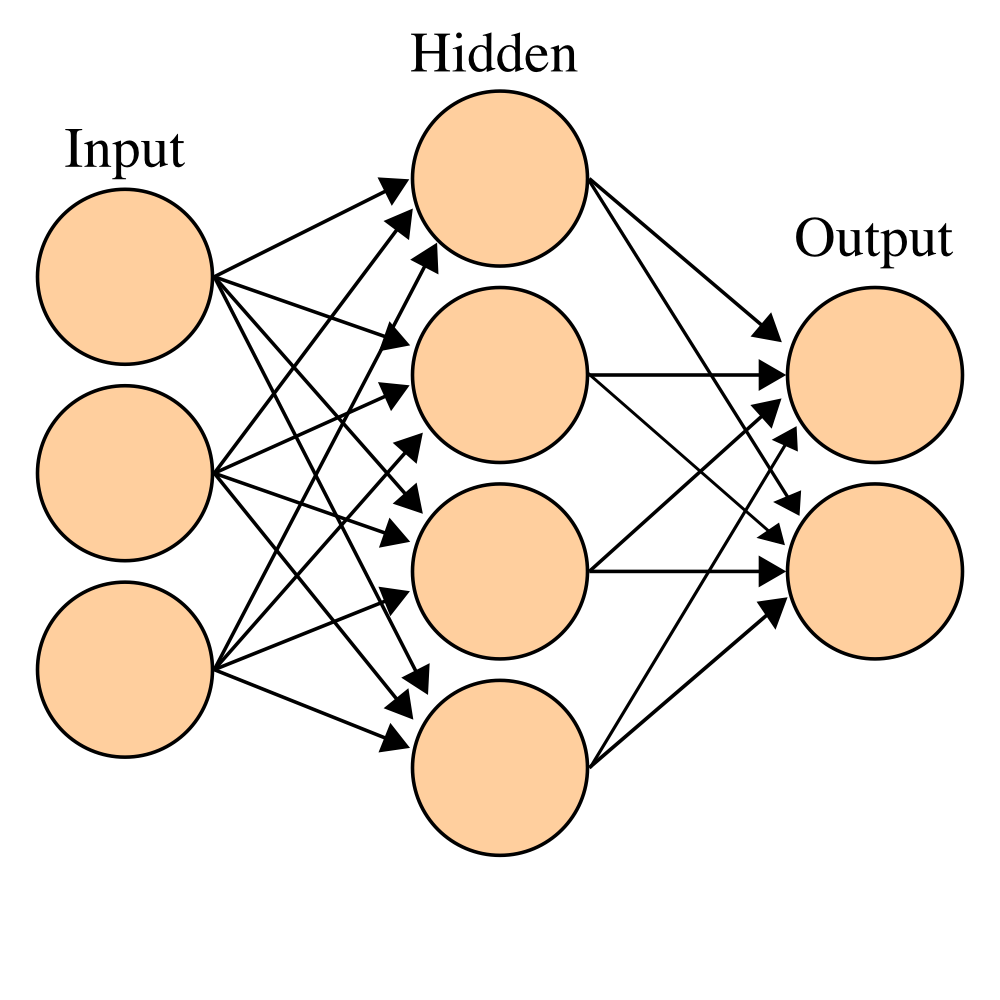
\includegraphics[scale=0.15]{Figures/ann.png}
    \caption{Example of ANN \cite{ann_wiki}}
    \label{fig:ann}
\end{figure}

\vspace*{0.33in}

\noindent Typically, a neural network is defined by three factors:
\begin{itemize}
    \item[1] How the different layers are interconnected
    \item[2] How the the weights are updated (learning process)
    \item[3] How the neuron's input value is converted to its output activation (activation function)
\end{itemize}

\section{Learning}
For every application the design of a neural network is different and after it has structured, the NN is ready to be trained. The first step is the initialization of the weigths. Normally they are initialized with random values, although, in \cite{yam2000weight} they developed a method to \textit{``determining the optimal initial weights of feedforward neural networks based on the Cauchy's inequality and a linear algebraic method''}. More, in \cite{fernandez2001weight} they tested seven different weights' initialization for twelve different problems. Thus, even the initialization of the connections values is application-dependant. \\
\noindent The learning paradigms can be grouped in three major categories: \textbf{supervised}, \textbf{unsupervised} and \textbf{reinforcement learning}.

\subsubsection{Supervised Learning}
This learning technique is the task of inferring a function from labeled training data \cite{sup_learn_wiki} \cite{mohri2012foundations}. The set responsible for training the model is composed by \textit{training examples} in which every sample consists of an \textit{input object} and a \textbf{desidered} \textit{output value}. What the algorithms does is to analyze the train dataset and produce an inferred function that will be used to map the new examples \cite{sup_learn_wiki}. Basically, the algorithm can be seen as \textit{learning} with a \textit{teacher}, in the sense that the there is costantly a feedback on the status of the application.

\subsubsection{Unsupervised Learning}
While in supervised learning, the system has a desidered output given from the training dataset, in the unsupervised paradigm, the system has to learn to estimate the right output given a new input \cite{ghahramani2004unsupervised}. In \textit{classification}, this output is a class label whereas in \textit{regression} is a real number. There are several ways to model this kind of learning system. \textit{Clustering}, using \textit{Self-Organizing Maps}, \textit{K-means} or \textit{hierachical clustering} are among the most famous approaches.

\subsubsection{Reinforcement Learning}
In reinforcement learning, the system takes actions to interact with its own environment. Each action will affect the state of the environment in which will produe a result in a form of either \textit{reward} or \textit{punishment}. The goal of this learning paradigm is to learn which is the best sequence of actions that maximises the rewards or minimises the punishments. There are quite a few approaches to find the best sequence of actions. The most famouse are \textit{Monte Carlo methods}, \textit{Temporal Difference methods} and \textit{Direct Policy search methods}.

\section{Multilayer Perceptron}
The model created by the Multilayer perceptron (MLP) serves to map a set of inputs onto a group of ouputs. The main feature of the MLP is that it a \textit{feedforward} artificial neural network. The MLP is formed by a defined number or layers in which every layer is \textit{fully connected} to following one. Every neuron of the network has a nonlinear activation function, with the exception of the input nodes. The techinque used in the MLP is of the kind of supervised and it uses the \textbf{backpropagation} for training the neurons \cite{mlp_wiki}. Backpropagation is discussed more in details in \ref{ssec:backprop}.

\subsubsection{Learning through Backpropagation} \label{ssec:backprop}
The learning phase in the neural network occurs in the moment that the connection weigths change based on the error value in the output. The error is calculated comparing the result the network produced with the expected one. This is a typical example of supervised learning because the network compares the result it just obtained with the one that it was expecting. This process is done through \textbf{backproagation}. \\

\noindent In backpropagation, the error output of the node $j$ in the $nth$ sample of the training dataset is given by
\begin{equation}
    e_{j}(n) = d_{j}(n) - y_{j}(n)
\end{equation}
where $d$ is the expected output whereas $y$ is the output value obtained from the neuron. The weights are then adjusted in such a way that the error is minimized. With \ref{eq:output_error} we are able to determine the corrections to apply given an output value produced by a perceptron.

\begin{equation}\label{eq:output_error}
    \varepsilon (n) = \frac{1}{2}\sum_{j} e^2_{j}(n)
\end{equation}

\noindent At this point using \ref{eq:gradient} we are able to determine the amount of change for each weight. This is done by \textbf{gradient descent} which is a first-order optimization algorithm. Gradient descent is used to find \textit{local minima} of a function, where \textit{"it takes steps proportionally to the negative of the gradient of the function in that point"}\cite{gradient_wiki}. The opposite instead, it means that it is approaching to the \textit{local maxima} of the function. ALthough, in this way, the process would be called \textit{gradient ascent}\cite{gradient_wiki}.

\begin{equation}\label{eq:gradient}
    \Delta w_{ji}(n) = -\eta \frac{\partial \varepsilon (n)}{\partial v_{j} (n)}y_{j}(n)
\end{equation}

\noindent In \ref{eq:gradient}, $\eta$ represents the \textit{learning rate} whereas $y_{i}$ is the output of the previous neuron \cite{mlp_wiki}. The learning rate parameter is one of the most importan parameters when design a neural network. The reason is that, the value used for it ensures that the weights are converging as fast as possible avoiding waivings. \\

\noindent The calculation of the derivates depends on the field $v_{j}$ where this value changes itself. Continuing, \ref{eq:gradient} can be simplified to \ref{eq:simpl_gradient} where $\phi^{\prime}$ represents the \textit{derivate} of the activation function described before. Note that this does not changes itself.

\begin{equation}\label{eq:simpl_gradient}
    \frac{\partial \varepsilon (n)}{\partial v_{j} (n)} = e_{j}(n)\phi^{\prime}(v_{j}(n))
\end{equation}

\section{Deep Learning}
\label{sec:deep_learning}
Deep Learning has several definitions in which those have been changing in last 10 years. Definition number 5 reported in \cite{deng2014deep} says the following: \textit{"Deep Learning is a new area of Machine Learning research, which has been introduced with the objective of moving Machine Learning closer to one of its original goals: Artificial Intelligence. Deep Learning is about learning multiple levels of representation and abstraction that help to make sense of data such as images, sound, and text."}.

\noindent There are two main aspects of the level of representations described above:
\begin{itemize}
    \item[1)] a model consists of several layers of nonlinear processing units
    \item[2)] for supervised and unsupervised approaches the feature representation have more abstract layers
\end{itemize}
\noindent It is possible to classify Deep Learning as an intersection between different research areas, such as: neural networks, pattern recognition, signal processing, etc..\cite{deng2014deep}

\subsection{Deep Neural Networs}
As described in \ref{sec:deep_learning}, a \textit{deep neural network} is composed by several hidden layers of perceptrons between the input(s) and the output(s) \cite{bengio2009learning}. As for the artificial neural networks, DNNs are able to model complex non-linear relationships. \cite{deep_learning_wiki}

\noindent Adding extra layers to a ANN permits to each layer to \textit{specialize} in solving a certain problem. For example, in \textit{visual pattern recognition} the neurons in the first layer can try to learn how to recognize edges in a picture, whereas those in the second layer might focus in learning ho to recognize more complex shapes like a square or a triangle built up from the previous edges. The next layers will try to learn even more complex shapes. In the case of speech recognition, we could split the problem in different parts as well. The first layer could focus in recognizing phonemes, the second layer can learn about the pitch voice, and so on.

\noindent The usage of multiple hidden layers gives to DNNs some advantages in learning how to solve complex problems compared to the shallow networks.\cite{dnn_website} An example of DNN is depicted in \ref{fig:deep_nn}.

\begin{figure}[!ht]
    \centering
    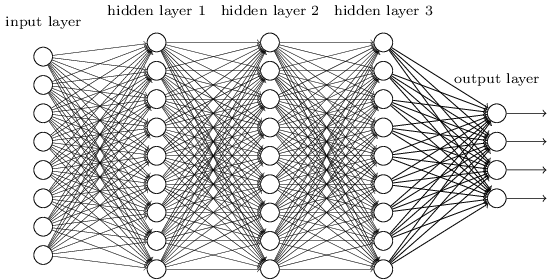
\includegraphics[scale=0.6]{Figures/deep_nn.png}
    \caption{Example of Deep Neural Network \cite{dnn_website}}
    \label{fig:deep_nn}
\end{figure}

\subsubsection{Architecture}
Deep Neural Networks are oftenly designed as feedforward networks and trained with the \textit{back propagation} algorithm. Although, to train acoustinc models for Automatic Speech Recognition (ASR) \textit{Convolutional Deep Neural Networks} (CNNs) presented better results than the typical feedforward design. Despite the similarity between the two networks, in CNNs \textit{"the neurons in the inputs of hidden units in layer m are from a subset of units in layer m-1, units that have spatially contiguous receptive fields"}. \cite{lenet}

\noindent To update the weights the \textit{stochastic gradient descent} is used as follow:

\begin{equation}
    w_{ij}(t+1) = w_{ij}(t) + \eta  \frac{\partial C}{\partial w_{ij}}
\end{equation}

\noindent where $\eta$ is the \textit{learning rate} whereas  $C$ is the \textit{cost function}. The activation function and the learning type have a direct influence in the choice of the cost function. For instance, a typical choice of the activation function for a supervised learning approach on a problem of multiclass classification are either \textbf{softmax function} or \textbf{cross entropy function}. The mathematical definition of \textit{softmax function} is defined in \ref{eq:softmax} where $p_{j}$ represents the class probability whereas $x_{k}$ and $x_{j}$ are the total input to neuron $x$ and $j$ of that layer. \textit{Cross entropy function} is defined by \ref{eq:cross_entropy} where $d_{j}$ is the target probability of the output neurons $j$ and $p_{j}$ is the probability output for $j$ after applying the activation function. \cite{deep_learning_wiki}

\begin{equation}\label{eq:softmax}
    p_{j} =  \frac{exp(x_{j})}{ \sum_k exp(x_{k})}
\end{equation}
\begin{equation}\label{eq:cross_entropy}
    C = -\sum_j d_{j}log(p_{j})
\end{equation}

\chapter{Implementation}
\label{chap:Implementation}
In this chapter we explain the infrastructure that performs all the necessary steps to produce an efficient feedback. A general overview is given and for each section, we describe in particular the tools as well as the way we manipulated the data in order to obtain the information useful for the user. The chapter is divided in two parts: the first part focuses on the back-end and the services we used to extract the features we described in \ref{chap:Speech Recognition}. The second part describe the front-end, that is, the \textit{Android}\footnote{\url{https://www.android.com}} application (called \textbf{PARLA}\footnote{\url{https://github.com/davideberdin/PARLA}}) with a particular focus on the feedback page and the general usage.

\section{General architecture}
\label{sec:general_architecture}

In \ref{fig:general_architecture} is shown the general architecture of the infrastructure.
The flow displays only the \textit{pronunciation testing} phase:

\begin{itemize}
	\item[1)] User says the sentence using the internal microphone of the smartphone (or through the headset)
	\item[2)] The application sends the audio file to the \textit{Speech Recognition service}
	\item[3)] The result of step 2 is sent to the \textit{Gaussian Mixture Model service}
	\item[4)] The result of step 3 is sent back to the application where a \textit{Feedback page} is displayed
	\item[5)] A short explanation for each chart is given to the user
	\item[6)] Back to step 1
\end{itemize}

\noindent The flow described above is the main feature of the whole project. Although, the application supplies other two important functionalities that are described more in detail in \ref{sec:android_app}. The first one is related to \textbf{critical listening} where the user is able to listen to the \textit{Native pronunciation} as well as to its one. This feature have a big impact on improving the pronunciation because it pushes the user to understand the differences as well as to emulate the way native speakers pronounce a specific sequence of words. The second feature regards the \textbf{history} (or progress). This page shows the trend of the user based on all the pronunciation he/she made during the usage of PARLA. The purpose of the history page is to help the user to see the progresses and to get an idea of how to improve the pronunciation. \\

\begin{figure}[!ht]
	\centering
	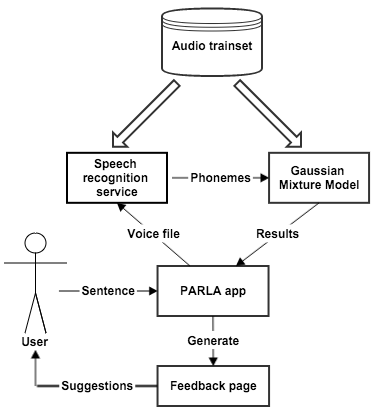
\includegraphics[scale=0.6]{Figures/general_architecture.png}
	\caption{General architecture of the infrastructure}
	\label{fig:general_architecture}
\end{figure}

\subsubsection{Implementation procedure}
\label{ssec:procedure}

Several step were made before to reach the architecture depicted in \ref{fig:general_architecture}. Generally speaking, we divided the implementation in two main categories: the first is composed by the \textit{data collection and training} phase whereas the second is formed by the \textit{mobile application} and \textit{server communication}. \\

\noindent The very first step was to collect the data from native speakers and apply some pre-processing techniques in such way that we were able to obtain only the information we needed to train the two services we had on the server.After the data collection, we trained both the models with the information we extracted in the previous step. The detailed procedures are described in \ref{ssec:training_sr_model} and \ref{ssec:training_gmm}. \\
\noindent When the training phase was completed, we set up the services and used \textit{REST} calls to communicate with the mobile application. These two parts were developed at the same time and are described in detail in \ref{sec:android_app}.


\section{Data collection}
\label{sec:data_collection}

The data collection step is a crucial phase of the entire project. The reason for such importance is that the audio record has to be clear, clean and as natural as possible. In fact, the people who participate to this phase were asked to pronounce the sentences as they would say in a day-by-day conversation. \\

\noindent We recorded 8 people divided in 4 males and 4 females at the University of Rochester using \textit{Audacity}\footnote{\url{http://audacityteam.org}}. Each person had to pronounce 10 sentences (see \ref{table:sentences}) and each sentence was pronounced 10 times. \\
\noindent The sentences were chosen in order to cover the most used English sounds and based on the frequencies of everyday usage\footnote{\url{http://www.learn-english-today.com/idioms/idioms_proverbs.html}}. 

\begin{table}[!ht]
	\centering
	\begin{tabular}{|c|c|}
		\hline
		\multicolumn{2}{|c|}{Sentences}      \\ \hline
		A piece of cake  & Fair and square   \\ \hline
		Blow a fuse      & Get cold feet     \\ \hline
		Catch some zs    & Mellow out        \\ \hline
		Down to the wire & Pulling your leg  \\ \hline
		Eager beaver     & Thinking out loud \\ \hline
	\end{tabular}
	\caption{Idioms used for testing the pronunciation}
	\label{table:sentences}
\end{table}

\noindent The total file we gathered were 800 and the average length of each file is \textbf{1s}. In total, we were able to gather 14 minutes of recorded audio. This amount of time was sufficient for training the speech recognition model and the GMM. In reality, for the speech recognition service, we initially trained the model with a bigger dataset and then we added the one with the sentences (details in \ref{fig:sphinx_service}). The reason is that the tool we used for the speech recognition, requires a large dataset\footnote{\url{http://cmusphinx.sourceforge.net/wiki/tutorialam}}.

\subsection{Data pre-processing}
\label{ssec:pre_processing}

The data pre-processing step is one of the most important procedure of the whole project. In fact, extracting the right information is crucial for both training the models and those voice-features that should be showed to the user. \\

\noindent The process starts by using the tool called \textbf{PRAAT}\footnote{http://www.fon.hum.uva.nl/praat/}. This tool is used for \textit{analysis of speech in phonetics} as well as for \textit{speech synthesis} and\textit{articulatory synthesis} \cite{boersma2001praat}. With PRAAT, we were able to analyze the audio files we collected in the very beginning of the project and extracting formants and stress. In \ref{sub:formants} and \ref{sec:stress} we detailed explained the meaning of these parameters. \\
From here, we generated a set of \textit{CSV} files where we saved the values of the formants and the stress for each audio file. These file are then used as input for a tool called \textbf{FAVE-Align}\cite{yuan2008speaker}. \\

\noindent FAVE-Align is a tool used for \textit{force alignment}. This process is used to determine where a particular word occurs in an audio frame \cite{forced_alignment_def}. In other words, FAVE-Align takes a text transcription and produce a PRAAT TextGrid file where it shows when those words start and end in the related audio file. In \ref{fig:fave-align_result}, there is an example of this procedure. The tool performs different phases in order to align audio and text.\\
The first step is to sample the audio file and apply the Fourier Transformation because there is the need to move from the \textit{time domain} to \textit{frequencies domain}. From here, the tool extract the \textit{spectrum} and apply the Inverse Fourier Transformation on it to obtain the so called \textbf{Cepstrum}. The \textit{cepstrum} is the representation in a small-window frame of the spectrum. Although, the amount of information extracted from the cepstrum are too high, and for this reason, the tool uses \textit{Perceptual Linear Prediction coefficients} to retrieve the necessary data to perform the alignment decision. These coefficients are used for feature extraction. The detailed process can be found at \cite{hermansky1990perceptual}. \\
The last part of this process is the decision making part and this is done by a \textit{Hidden Markov Model}. \\ 

\begin{figure}[!ht]
	\centering
	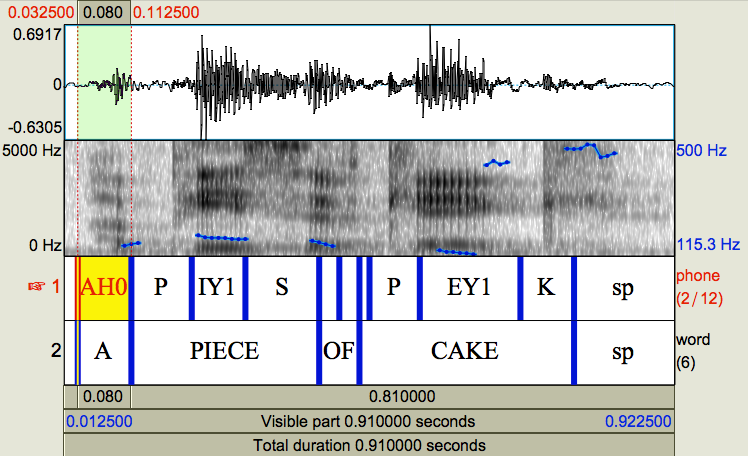
\includegraphics[scale=0.5]{Figures/fave_align.png}
	\caption{Result from FAVE-Align tool opened in PRAAT}
	\label{fig:fave-align_result}
\end{figure}

\noindent The outcome of the previous step is used as input for the tool called \textbf{FAVE-Extract}. This tool helps to automates the vowel formant analysis. The process is dived in two main steps: the first is finding the \textit{Measurement Points} and the second is the \textit{Remeasurement}. \\
In \cite{rosenfelder2011fave} is explained that for most vowels it is possible to find the measurement point by listening 1/3 of the total duration. This point is necessary for determining the identity of the vowel, that is, the name of the vowel itself. For more complex vowels, a different approach is done, that is, the point is halfway between the F1 (main formant) maximum value and the beginning of the segment. In addition, the LPC analysis is performed on both beginning and end of the vowel in order to pad the vowel's window. This \emph{ensure a formant track through the full vowel’s duration}\cite{harrison2004variability}. The result of this step is a set of candidates. This set is composed by the potential formants estimated from the likelihood of the \textbf{ANAE} distribution. The \textit{Atlas of North American English} (ANAE) is the set of phonology formants values depending on the English regional area. The winner formant is determined by the Posterior probability. This step does not take in consideration the provenience of the speaker. \\

\noindent The second part of the formants extraction tool is to remeasure the parameters by adjusting the ANAE distribution based on the regional area of the speaker. In this way, the formant value will be more accurate. An example of result from FAVE-Extract is shown in \ref{fig:fave-extract_example}.

\begin{figure}[!ht]
	\centering
	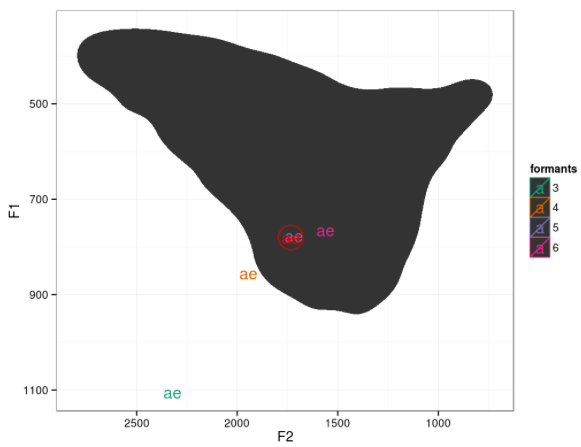
\includegraphics[scale=0.5]{Figures/fave-extract_example.png}
	\caption{Result from FAVE-Extract}
	\label{fig:fave-extract_example}
\end{figure}

\noindent The result of the data pre-processing is a set of information composed by the average value of F1 and F2 formants with their respectively vowels text representation. The formants values will be then used to train both the speech recognition model and the Gaussian Mixture Model.

\section{Server}
\label{sec:server}

The back-end system is divided in two different services: the first one handles the speech recognition converting the user's voice into a set of phonemes, whereas the second service is in charged of all the other operations a user can do, such as login/logout, history data, vowels prediction system, usage collection, etc.. This section explains more in detail how we extract the information from the audio files and how we manipulate those before to give the feedback to the user.

\subsection{Training the Speech Recognition model} 
\label{ssec:training_sr_model}

goofy

\begin{figure}[!ht]
	\centering
	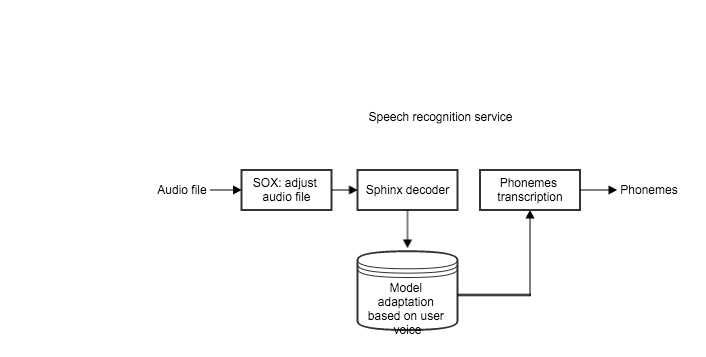
\includegraphics[scale=0.6]{Figures/sphinx_service.png}
	\caption{Architecture of the Speech recognition service}
	\label{fig:sphinx_service}
\end{figure}

\subsection{Training the Gaussian Mixture Model}
\label{ssec:training_gmm}

goofy

\begin{figure}[!ht]
	\centering
	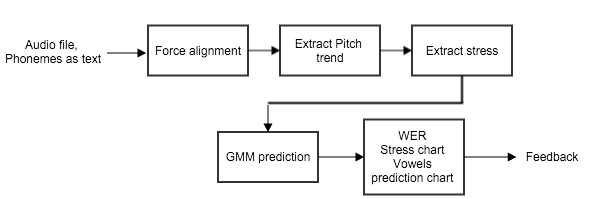
\includegraphics[scale=0.6]{Figures/gmm_service.png}
	\caption{Architecture of the Gaussian Mixture Model service}
	\label{fig:gmm_service}
\end{figure}


%%%%%%%%%%%%%%%%%%%%%%%%%%%%%%%%%%%%%%%%%%%%%%%%%%%%%%%%%%%%%%%%%%%%%%%%%%%%%%%%
%%%%%							ANDROID PART							   %%%%%
%%%%%%%%%%%%%%%%%%%%%%%%%%%%%%%%%%%%%%%%%%%%%%%%%%%%%%%%%%%%%%%%%%%%%%%%%%%%%%%%


\section{Android application}
\label{sec:android_app}

\subsection{Layouts}
\label{ssec:layouts}

\subsection{Feedback layout}
\label{ssec:feedback_layout}

\subsection{Usage procedure}
\label{ssec:usage_procedure}
\chapter{User studies and Results}
\label{chap:results}

The results of this study were determined by the answers of a survey completed by the users that participate to the testing phase. \\
\noindent We recruited 6 people from Uppsala University and asked them to use the application for a period of 2 weeks and fill up a survey with 26 questions (see Appendix). The survey is anonymous and divided in 3 sections: the first part was designed to gather the information related to the audience. The second part aimed to rate the interest in learning a new language using a mobile device, whereas the third part was dedicated to the application itself. \\

\subsection*{Audience}
\label{sub:Audience}

This section presents the answers related to the users personal information to get a better understaning of the audience. From \ref{fig:gender_chart} and \ref{fig:age_chart} we can say that the majority of our users are male and between the age of 24-29 years old.  Table \ref{table:native_languages} describes the native language of the users.

\begin{figure}[!ht]
	\centering
	\begin{minipage}{.5\textwidth}
		\centering
		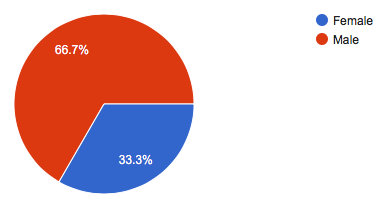
\includegraphics[scale=0.5]{Figures/responses/audience_gender.png}
		\caption{Gender chart}
		\label{fig:gender_chart}
	\end{minipage}%
	\begin{minipage}{.5\textwidth}
		\centering
		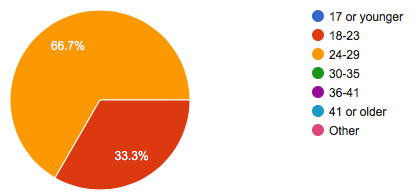
\includegraphics[scale=0.5]{Figures/responses/audience_age.png}
		\caption{Age chart}
		\label{fig:age_chart}
	\end{minipage}
\end{figure}

\begin{table}[!ht]
    \centering
    \begin{tabular}{|l|c|}
        \hline
        \multicolumn{1}{|c|}{\textbf{Native language}} & \textbf{Amount} \\ \hline
        Italian                                        & 2               \\ \hline
        Greek                                          & 2               \\ \hline
        Swedish                                        & 1               \\ \hline
        Arabic                                         & 1               \\ \hline
    \end{tabular}
    \caption{Users native languages}
    \label{table:native_languages}
\end{table}

\noindent All testers were students from the Computer Science department as well as comfortable in using mobile applications on a daily base.

\subsection*{Interest}
\label{sub:Interest}

This section describes the interest of our testers in learning and improving a new language using a mobile application instead of the traditional student-teacher class. Results are vey positive and we can confirm that the interest is high. In particular, avoiding the interaction with a physical teacher is very welcomed.

\begin{figure}[!ht]
	\centering
	\begin{minipage}{.5\textwidth}
		\centering
		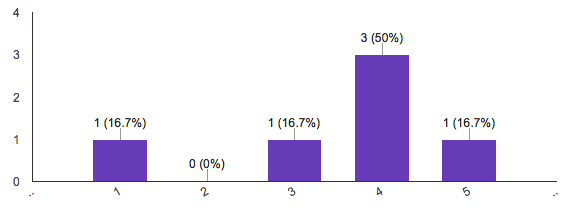
\includegraphics[scale=0.5]{Figures/responses/interest_improving_lang.png}
		\caption{Interest in improving English language}
		\label{fig:int_improving_lang}
	\end{minipage}%
	\begin{minipage}{.5\textwidth}
		\centering
		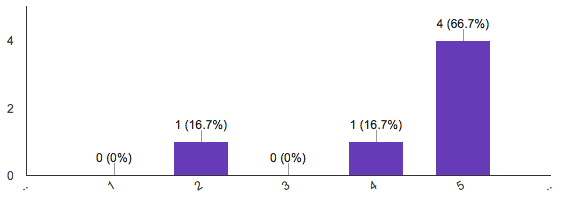
\includegraphics[scale=0.5]{Figures/responses/interest_learning_language.png}
		\caption{Interest in learning a new language}
		\label{fig:int_learnign_lang}
	\end{minipage}
    \begin{minipage}{.5\textwidth}
        \centering
        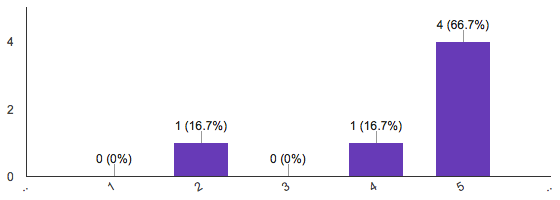
\includegraphics[scale=0.5]{Figures/responses/interest_usage_smartphone.png}
        \caption{Interest in using a smartphone}
        \label{fig:int_usage_smartphone}
    \end{minipage}%
\end{figure}
\begin{figure}[!ht]
	\centering
	\begin{minipage}{.5\textwidth}
		\centering
		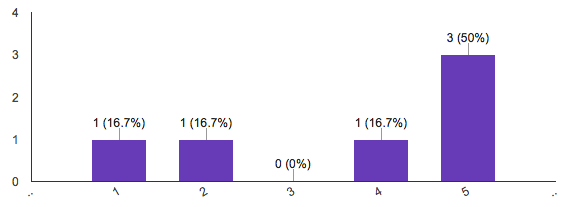
\includegraphics[scale=0.5]{Figures/responses/interest_visual_feedback.png}
		\caption{Interest in having visual feedback}
		\label{fig:int_visual_feedbak}
	\end{minipage}%
	\begin{minipage}{.5\textwidth}
		\centering
		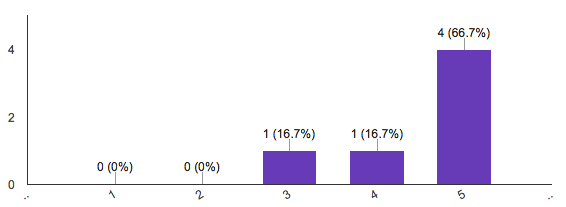
\includegraphics[scale=0.5]{Figures/responses/interest_no_teacher.png}
		\caption{Interest in not having a teacher's supervision}
		\label{fig:int_no_teacher}
	\end{minipage}
\end{figure}


\subsection*{Application}
\label{sub:Application}

\begin{figure}[!ht]
	\centering
	\begin{minipage}{.5\textwidth}
		\centering
		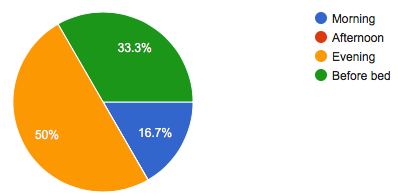
\includegraphics[scale=0.5]{Figures/responses/application_period_of_usage.png}
		\caption{Moment of the day}
		\label{fig:int_improving_lang}
	\end{minipage}%
	\begin{minipage}{.5\textwidth}
		\centering
		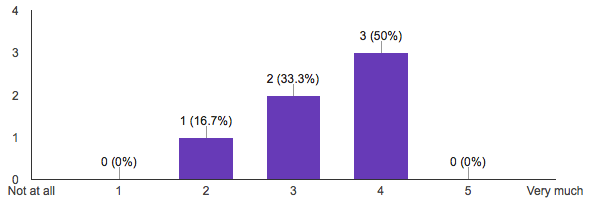
\includegraphics[scale=0.5]{Figures/responses/application_liked.png}
		\caption{General appreciation}
		\label{fig:int_usage_smartphone}
	\end{minipage}%
\end{figure}

\begin{figure}[!ht]
	\centering
	\begin{minipage}{.5\textwidth}
		\centering
		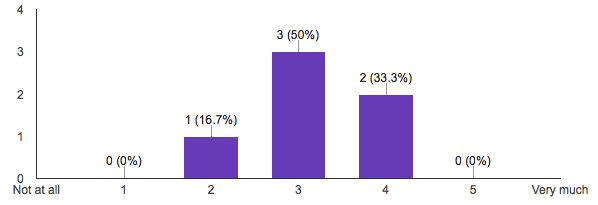
\includegraphics[scale=0.5]{Figures/responses/application_usage.png}
		\caption{Interest in continuing using the application}
		\label{fig:int_improving_lang}
	\end{minipage}%
	\begin{minipage}{.5\textwidth}
		\centering
		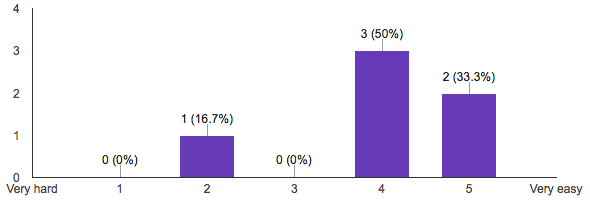
\includegraphics[scale=0.5]{Figures/responses/application_usage_difficulty.png}
		\caption{Usage difficulty}
		\label{fig:int_learnign_lang}
	\end{minipage}
\end{figure}

Here all the understandings

\begin{figure}[!ht]
	\centering
	\begin{minipage}{.5\textwidth}
		\centering
		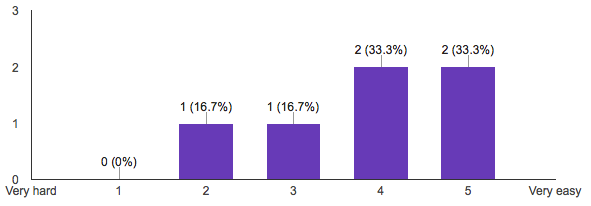
\includegraphics[scale=0.5]{Figures/responses/understanding_main.png}
		\caption{Understanding the main page}
		\label{fig:int_improving_lang}
	\end{minipage}%
	\begin{minipage}{.5\textwidth}
		\centering
		\includegraphics[scale=0.5]{Figures/responses/understanding_listening.png}
		\caption{Understanding the critical listening page}
		\label{fig:int_learnign_lang}
	\end{minipage}
	\begin{minipage}{.5\textwidth}
		\centering
		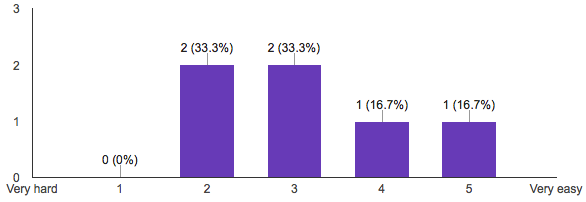
\includegraphics[scale=0.5]{Figures/responses/understanding_feedback.png}
		\caption{Understanding feedback page}
		\label{fig:int_usage_smartphone}
	\end{minipage}%
\end{figure}

\begin{figure}[!ht]
	\centering
	\begin{minipage}{.5\textwidth}
		\centering
		\includegraphics[scale=0.5]{Figures/responses/understanding_stress.png}
		\caption{Understanding stress on a sentence}
		\label{fig:int_improving_lang}
	\end{minipage}%
	\begin{minipage}{.5\textwidth}
		\centering
		\includegraphics[scale=0.5]{Figures/responses/understanding_pitch.png}
		\caption{Understanding pitch trend}
		\label{fig:int_learnign_lang}
	\end{minipage}
	\begin{minipage}{.5\textwidth}
		\centering
		\includegraphics[scale=0.5]{Figures/responses/understanding_vowels.png}
		\caption{Understanding vowels chart}
		\label{fig:int_usage_smartphone}
	\end{minipage}%
\end{figure}

\begin{figure}[!ht]
	\centering
	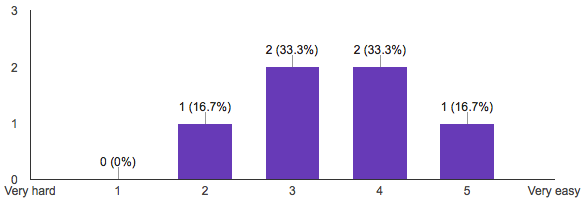
\includegraphics[scale=0.5]{Figures/responses/understanding_history.png}
	\caption{Understanding history page}
	\label{fig:int_improving_lang}
\end{figure}

Actual results

\begin{figure}[!ht]
	\centering
	\begin{minipage}{.5\textwidth}
		\centering
		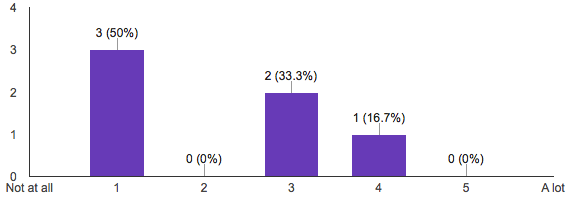
\includegraphics[scale=0.5]{Figures/responses/application_improved_pronunciation.png}
		\caption{Pronunciation improved}
		\label{fig:int_improving_lang}
	\end{minipage}%
	\begin{minipage}{.5\textwidth}
		\centering
		\includegraphics[scale=0.5]{Figures/responses/utility_of_listening.png}
		\caption{Utility of critical/self listening}
		\label{fig:int_learnign_lang}
	\end{minipage}
	\begin{minipage}{.5\textwidth}
		\centering
		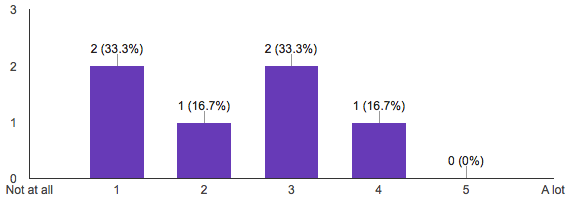
\includegraphics[scale=0.5]{Figures/responses/application_rate_feedback.png}
		\caption{Utility of feedback}
		\label{fig:int_usage_smartphone}
	\end{minipage}%
\end{figure}

\begin{figure}[!ht]
	\centering
	\includegraphics[scale=0.5]{Figures/responses/utility_of_history.png}
	\caption{Utility of history page}
	\label{fig:int_usage_smartphone}
\end{figure}%
\chapter{Conclusions}
\label{chap:Conclusions}

\chapter{Future Works}
\label{ch:Future Works}

Given the results many other applications can be extracted from this prototype. Smartwatches for example, are becoming the next hot-platform for developing new applications. In fact, it is possible to extend this product in such a way that a user can practice day-by-day by simply using the internal microphone of the smartwatch. The procedure and the time taken for the whole process is less then using a common smartphone. Of course, the whole feedback system has to be redesigned and scaled to be able to fit the information in a smaller screen. \\

\noindent Another interesting way for pushing the limits of this application, is to make it more challenging more like a video game. In fact, provide the opportunity for the user to challenge other users should give a psychological boost for improving the pronunciation and be better than other competitors. Thus, the usage of achievements, objectives, etc. will involve the user in a completely different experience but still with the intent of improving the pronunciation. \\

\noindent \textit{Google Glass}\footnote{https://www.google.com/glass/start/}, \textit{Microsoft HoloLens}\footnote{https://www.microsoft.com/microsoft-hololens/en-us}, \textit{Oculus Rift}\footnote{https://www.oculus.com/en-us/} and other augmented reality devices, could be used for language learning process. The user will then be involved in an experience that would be closer to an actual lecture with a qualified teacher. Using a virtual assistant and a complex AI system, it would be possible to reproduce this old, but still very effective, way of learning. At the same time, interaction with other users that have the same application and device, would be incredibly effective to train not only the pronunciation but also grammar, reading-comprehension and conversation. \\

\noindent The number of possible and future applications is incredibly large. These were simple example of how we can use the new coming technology in the world of learning languages.


%%%%%% Bibliography %%%%%%
{
	\bibliographystyle{ieeetr}
	\bibliography{bibliography}
}

\pagenumbering{gobble}
\begin{appendices}

\begin{landscape}
	\begin{figure}[!ht]
		\caption{BIC results for GMM selection}	
		\label{fig:bic1}			
		\begin{tabular}{ccccc}
			\subfloat{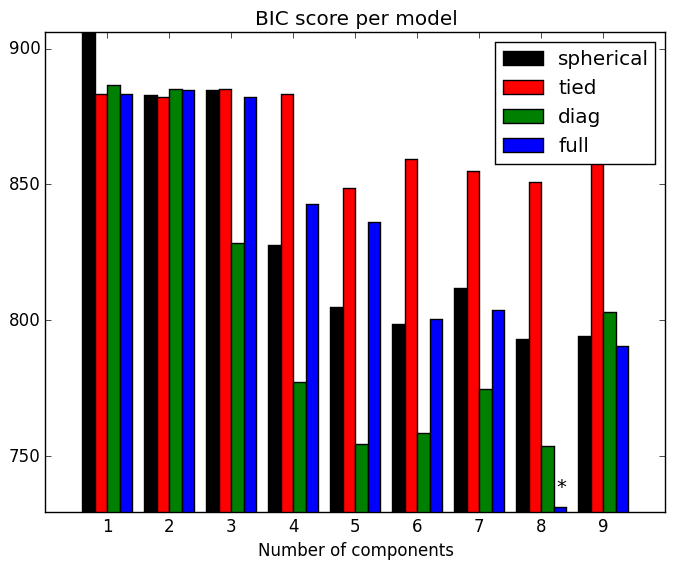
\includegraphics[scale=0.25]{Figures/bic/bic_0.png}} & 
			\subfloat{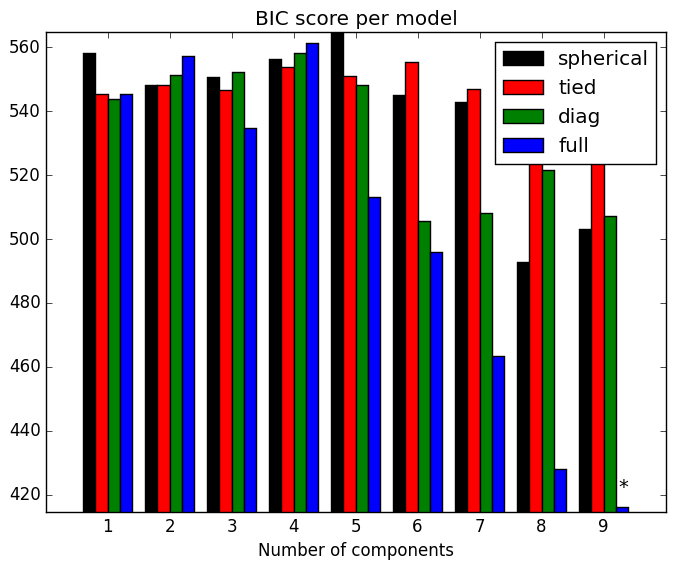
\includegraphics[scale=0.25]{Figures/bic/bic_1.png}} & 
			\subfloat{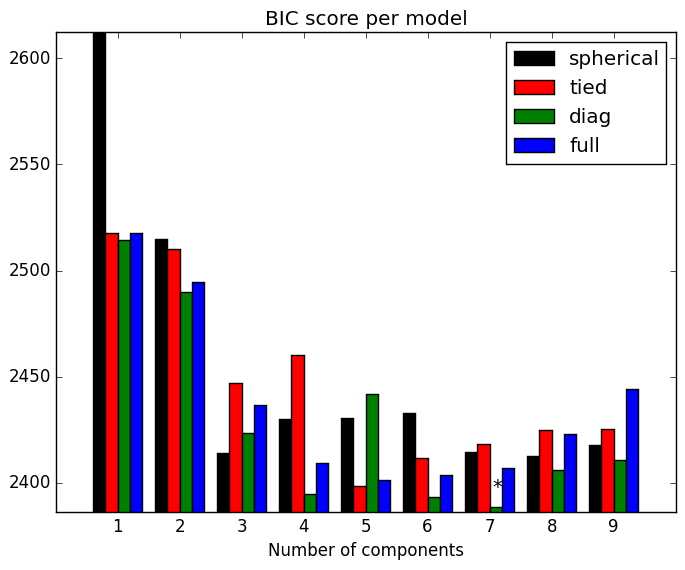
\includegraphics[scale=0.25]{Figures/bic/bic_2.png}} &		
			\subfloat{\includegraphics[scale=0.25]{Figures/bic/bic_3.png}} & 
			\subfloat{\includegraphics[scale=0.25]{Figures/bic/bic_4.png}} \\ 
			
			\subfloat{\includegraphics[scale=0.25]{Figures/bic/bic_5.png}} &			
			\subfloat{\includegraphics[scale=0.25]{Figures/bic/bic_6.png}} & 
			\subfloat{\includegraphics[scale=0.25]{Figures/bic/bic_7.png}} & 
			\subfloat{\includegraphics[scale=0.25]{Figures/bic/bic_8.png}} &			
			\subfloat{\includegraphics[scale=0.25]{Figures/bic/bic_9.png}} \\
			
			\subfloat{\includegraphics[scale=0.25]{Figures/bic/bic_10.png}} & 
			\subfloat{\includegraphics[scale=0.25]{Figures/bic/bic_11.png}} &			
			\subfloat{\includegraphics[scale=0.25]{Figures/bic/bic_12.png}} & 
			\subfloat{\includegraphics[scale=0.25]{Figures/bic/bic_13.png}} & 
			\subfloat{\includegraphics[scale=0.25]{Figures/bic/bic_14.png}} \\
			
			\subfloat{\includegraphics[scale=0.25]{Figures/bic/bic_15.png}} & 
			\subfloat{\includegraphics[scale=0.25]{Figures/bic/bic_16.png}} & 
			\subfloat{\includegraphics[scale=0.25]{Figures/bic/bic_17.png}} &
			\subfloat{\includegraphics[scale=0.25]{Figures/bic/bic_18.png}} & 
			\subfloat{\includegraphics[scale=0.25]{Figures/bic/bic_19.png}} \\			
		\end{tabular}
	\end{figure}
\end{landscape}

\begin{landscape}
	\begin{figure}[!ht]
		\caption{BIC results for GMM selection}
		\label{fig:bic2}
		\begin{tabular}{ccccc}			 
			\subfloat{\includegraphics[scale=0.25]{Figures/bic/bic_20.png}} &		
			\subfloat{\includegraphics[scale=0.25]{Figures/bic/bic_21.png}} & 
			\subfloat{\includegraphics[scale=0.25]{Figures/bic/bic_22.png}} & 
			\subfloat{\includegraphics[scale=0.25]{Figures/bic/bic_23.png}} &
			\subfloat{\includegraphics[scale=0.25]{Figures/bic/bic_24.png}} \\
			
			\subfloat{\includegraphics[scale=0.25]{Figures/bic/bic_25.png}} & 
			\subfloat{\includegraphics[scale=0.25]{Figures/bic/bic_26.png}} &
			\subfloat{\includegraphics[scale=0.25]{Figures/bic/bic_27.png}} & 
			\subfloat{\includegraphics[scale=0.25]{Figures/bic/bic_28.png}} & 
			\subfloat{\includegraphics[scale=0.25]{Figures/bic/bic_29.png}} \\
			
			\subfloat{\includegraphics[scale=0.25]{Figures/bic/bic_30.png}} & & & &
		\end{tabular}
	\end{figure}
\end{landscape}
\includepdf[pages=-]{Chapters/survey_app.pdf}
%\chapter{Surveys}
\label{ch:surveys}

here the surveys
\end{appendices}
\mbox{} 
\thispagestyle{empty} 
\clearpage


\topskip0pt
\vspace*{\fill}
\begin{em}
	\noindent Viagiar desc\`{a}nta, ma chi parte mona torna mona \\
	\textbf{Old Venetian aphorism}
\end{em}	
\vspace*{\fill}

\end{document}
